%!TEX spellcheck=en-US
\documentclass[aspectratio=169]{beamer} % aspectratio={169,43}

\usepackage[english]{babel} % define language

\usetheme[%
  titlepage=split, % options={center,split}, default=center
  headline=sectionsubsection, % options={empty,section,sectionsubsection}, default=sectionsubsection
  sectionpage=true, %options={true,false}, default=true
  ]{LAMCOS} % load theme

% Load bibliography file to access citation keys
\addbibresource{Biblio_YETI.bib}

%-------------------------------------------------------------------------------
% INFO
\title[Optim IGA]{ L'analyse isogéométrique pour l'optimisation de forme}
\author[A. Duval]{%
  Arnaud Duval\textsuperscript{1}
  % A. Author\textsuperscript{1}, B. Bauthor\textsuperscript{2}, C. Cauthor\textsuperscript{1}
}
\institute[LaMCoS]{%
  \textsuperscript{1}LaMCoS\,: Laboratoire de Mécanique des Contacts et des Structures,\\
  CNRS, INSA Lyon, LaMCoS, UMR5259, Villeurbanne, France\\
  % \textsuperscript{2}Name of another institute, very long adress on a cool street, in a very beautiful city
}
\date[15/05/25]{15 mai 2025}

\logo{%
  \pgfuseimage{lamcos}%
  % to add other logos and put them side-by-side uncomment below
  % \begin{pgfpicture}
  %     \pgftext[at=\pgfpoint{0cm}{0cm},right]{\pgfuseimage{lamcos}}
  %     \pgftext[at=\pgfpoint{0.5cm}{0cm},left]{\pgfuseimage{other-logo}}
  %   \end{pgfpicture}
  % change other-logo declaration in beamerthemeLAMCOS.sty
  }

% \sectiongraphic{images/Toucan.jpg} % to remove the section graphic, simply comment this line
%-------------------------------------------------------------------------------


%-------------------------------------------------------------------------------
% CUSTOM COMMANDS AND PACKAGES
% import your own package or define custom commands here
\usepackage{fontawesome}
% \newcommand{\command}[1]{#1}
\newcommand\blfootnote[1]{%
  \begingroup
  \renewcommand\thefootnote{}\footnote{#1}%
  \addtocounter{footnote}{-1}%
  \endgroup
}

% \newcommand{\includepdft}[2]{%
%   \begingroup
%     \def\includegraphics[##1]##2{\includegraphics[width=#2]{##2}}%
%     \input{#1.pdf_t}%
%   \endgroup
% }
%-------------------------------------------------------------------------------


%-------------------------------------------------------------------------------
% DOCUMENT

\begin{document}

\maketitle

\section*{Introduction}

% \tableofcontents


\begin{frame}
  \frametitle{Conception assistée par ordinateur}
  \only<1->{
  \faHandORight{} Dialogue conception / calcul traditionnel
  \begin{center}
    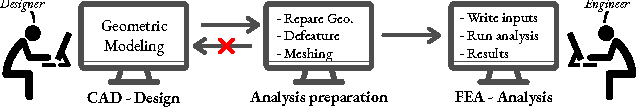
\includegraphics[width=0.8\linewidth]{figures/tradional_process.pdf} \\
      Préparation du modèle pour l'analyse {\bf $\approx$ 90\% du temps}
  \end{center}}
  \only<2>{
  \begin{center}
    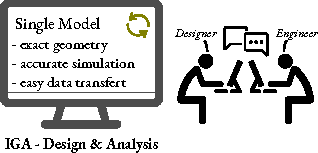
\includegraphics{figures/IGA_process.pdf}
  \end{center}}
  \blfootnote{Illustrations : T. Hirschler} \\
\end{frame}

\begin{frame}
  \frametitle{Optimisation de forme}
  \begin{center}
    \includegraphics<1>[width=0.67\linewidth]{figures/a-typeOfOpt.pdf}
    \includegraphics<2>[width=0.67\linewidth]{figures/b-typeOfOpt.pdf}
  \end{center}
  \blfootnote{Illustrations : T. Hirschler}
\end{frame}

\begin{frame}
  \frametitle{Optimisation de forme}
  \begin{block}{Ingrédients}
    \begin{itemize}
      \item Bonne représentation de la géométrie
      \item Modèle d'analyse efficace
      \item Lien fort entre la géométrie et l'analyse
    \end{itemize}
    \only<2>{\faHandORight{} {\bf L'analyse isogéométrique offre (promet) tout ça !}}
  \end{block}
\end{frame}

\section[Géométrie]{Analyse iso{\bf GÉOMÉTRIQUE}}

\begin{frame}
  \frametitle{Analyse isogéométrique}
  L'analyse isogéométrique se base sur les primitives géométriques issues de la CAO (B-Splines, NURBS, \dots).
  Elle inclut la méthode des éléments finis comme un cas particulier \cite{cottrell_isogeometric_2009}.
  \begin{columns}
    \begin{column}{0.22 \linewidth}
      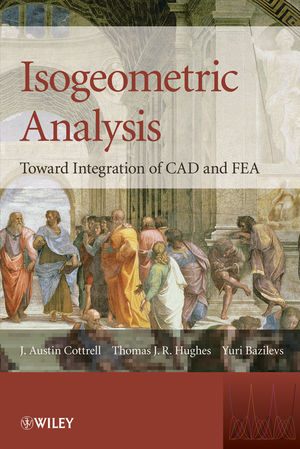
\includegraphics[width=\linewidth]{figures/Cottrel.jpg}
    \end{column}

    \begin{column}{0.6\linewidth}
      \only<1>{
        \begin{itemize}
            \item Modélisation géométrique précise
            \item Raffinement de maillage simple
            \item {\color{LAMCOSgreen} Fonctions de forme régulières}
            \item Meilleur capacité d'approximation
            \item {\color{LAMCOSgreen} Champs dérivés précis}
        \end{itemize}
      }
      \only<2>{
        \begin{itemize}
          \item Raffinement local impossible en B-splines (structure de {\color{LAMCOSred} produit tensoriel})
          \item {\color{LAMCOSred} Verrouillage} présent pour des degrés polynomiaux modérés
          \item Pas/peu d'intégration dans les codes commerciaux
          \item {\color{LAMCOSred} Lien CAO/calcul difficile en 3D} (modèle B-Rep, courbes de trim, \dots)
        \end{itemize}
      }
    \end{column}
  \end{columns}
\end{frame}

\begin{frame}
  \frametitle{Modèle CAO .vs. modèle IGA}
  \begin{itemize}
    \item Approche B-rep pour les volumes
  \end{itemize}
  \begin{center}
    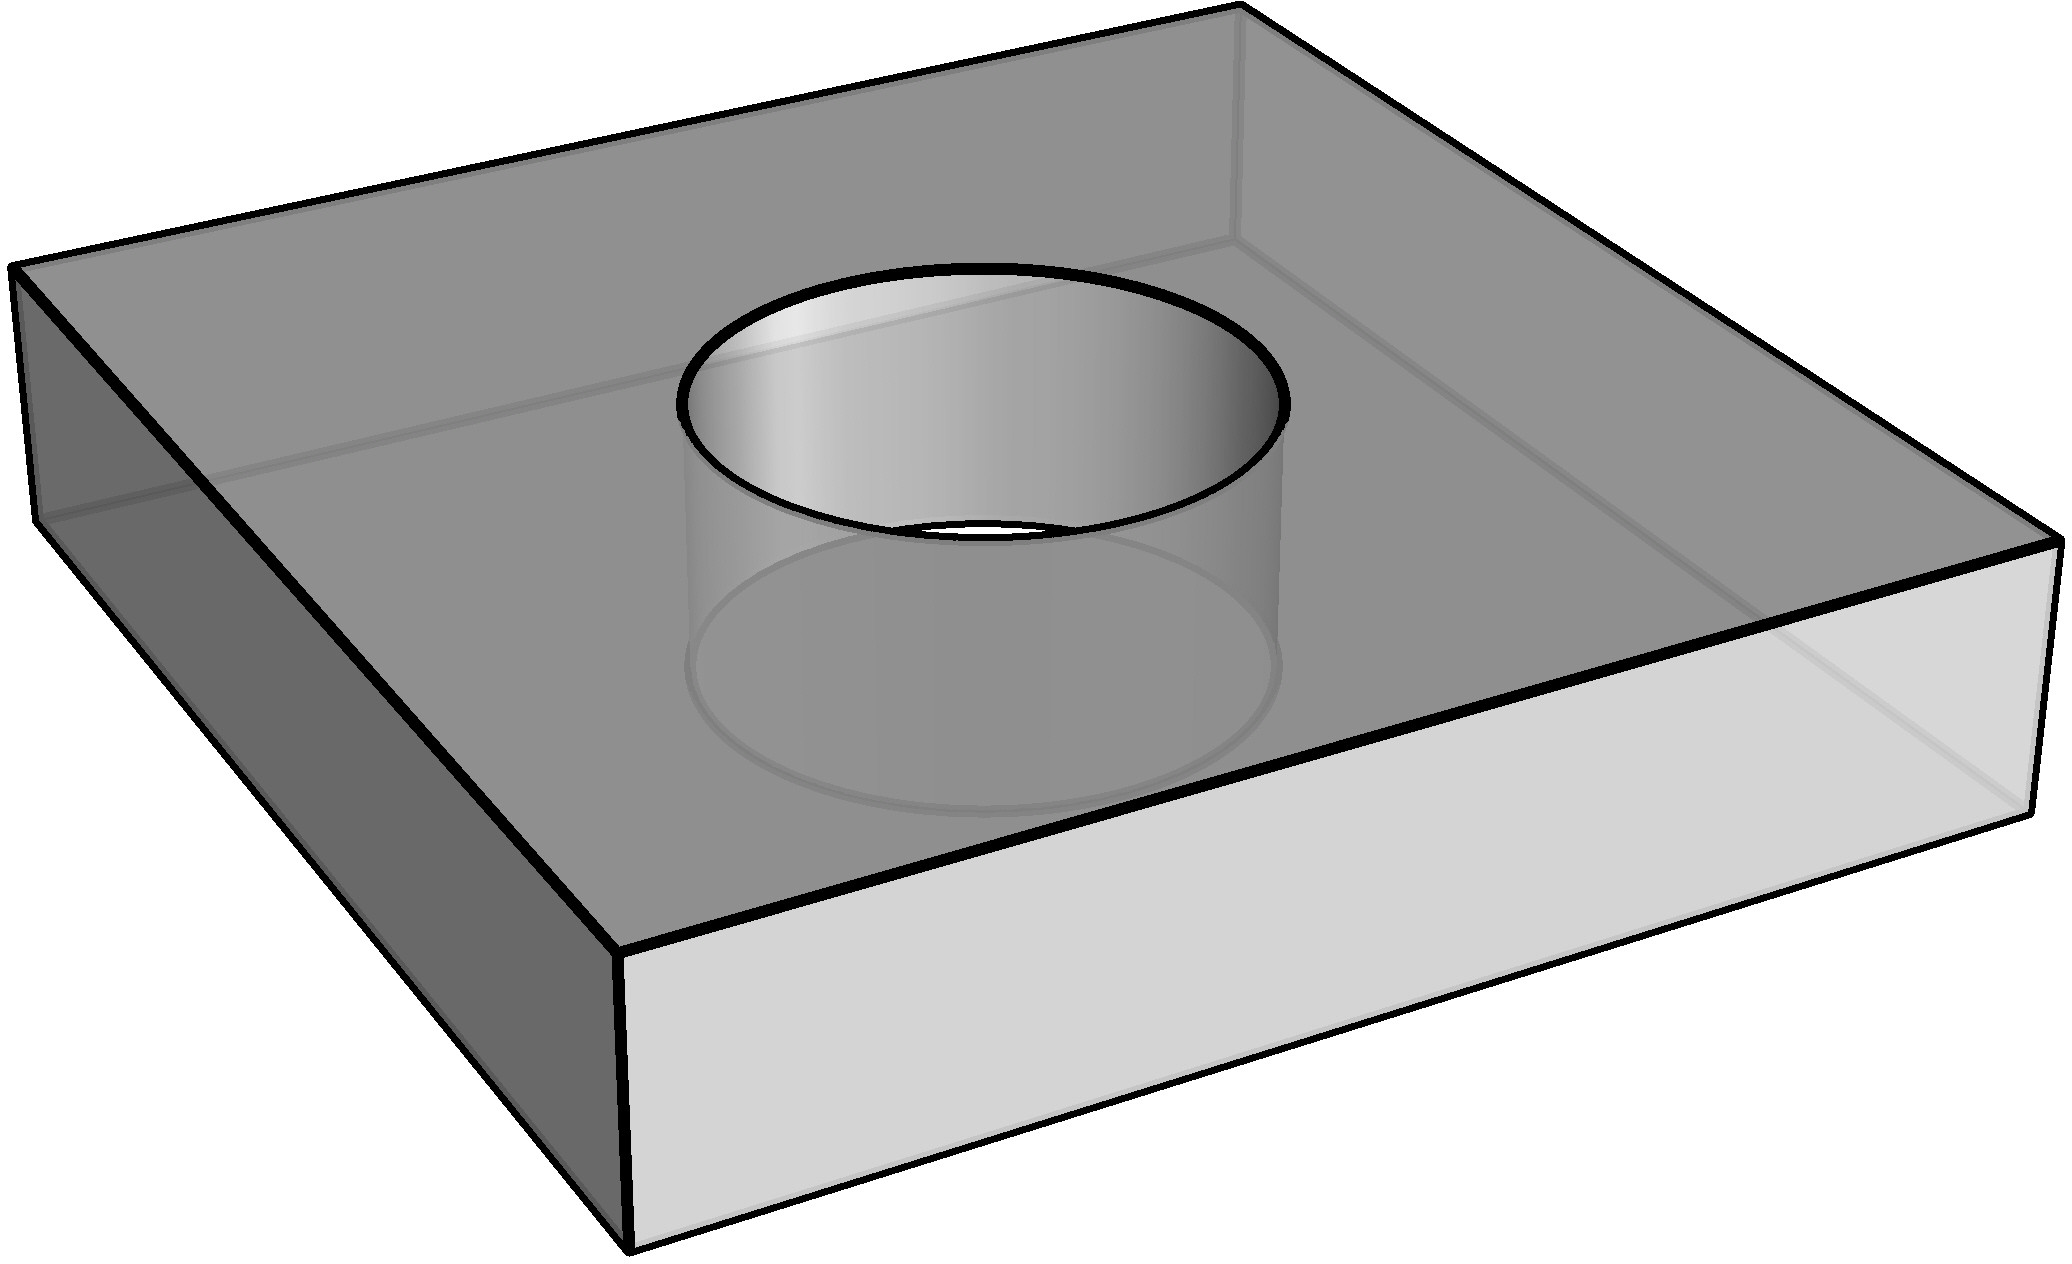
\includegraphics[height=2.5cm]{figures/CAD_01.jpg}
    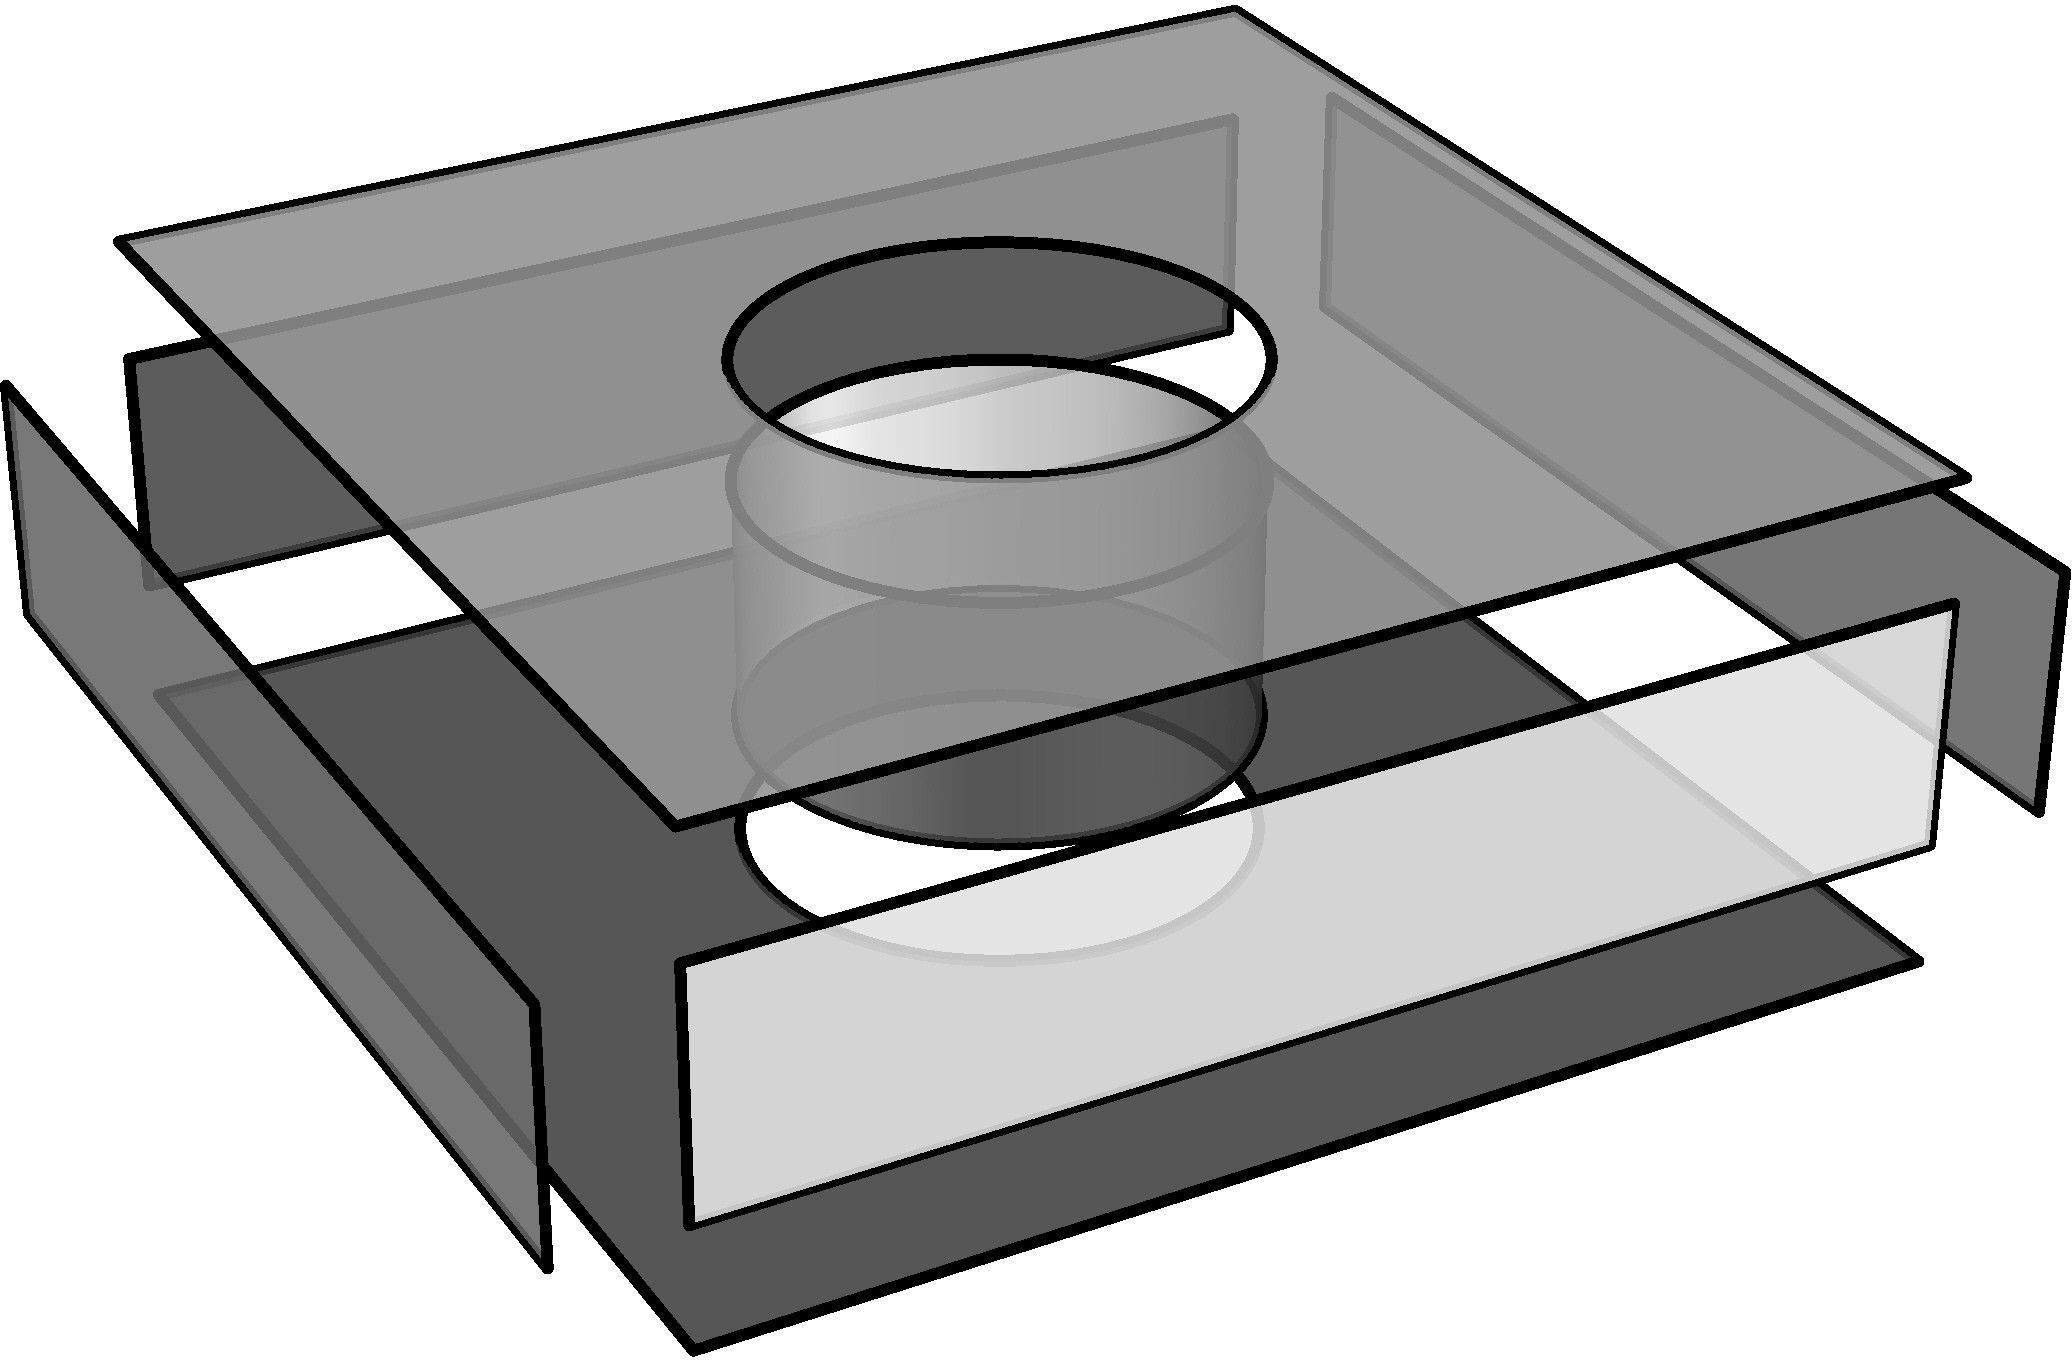
\includegraphics[height=2.5cm]{figures/CAD_02.jpg}
    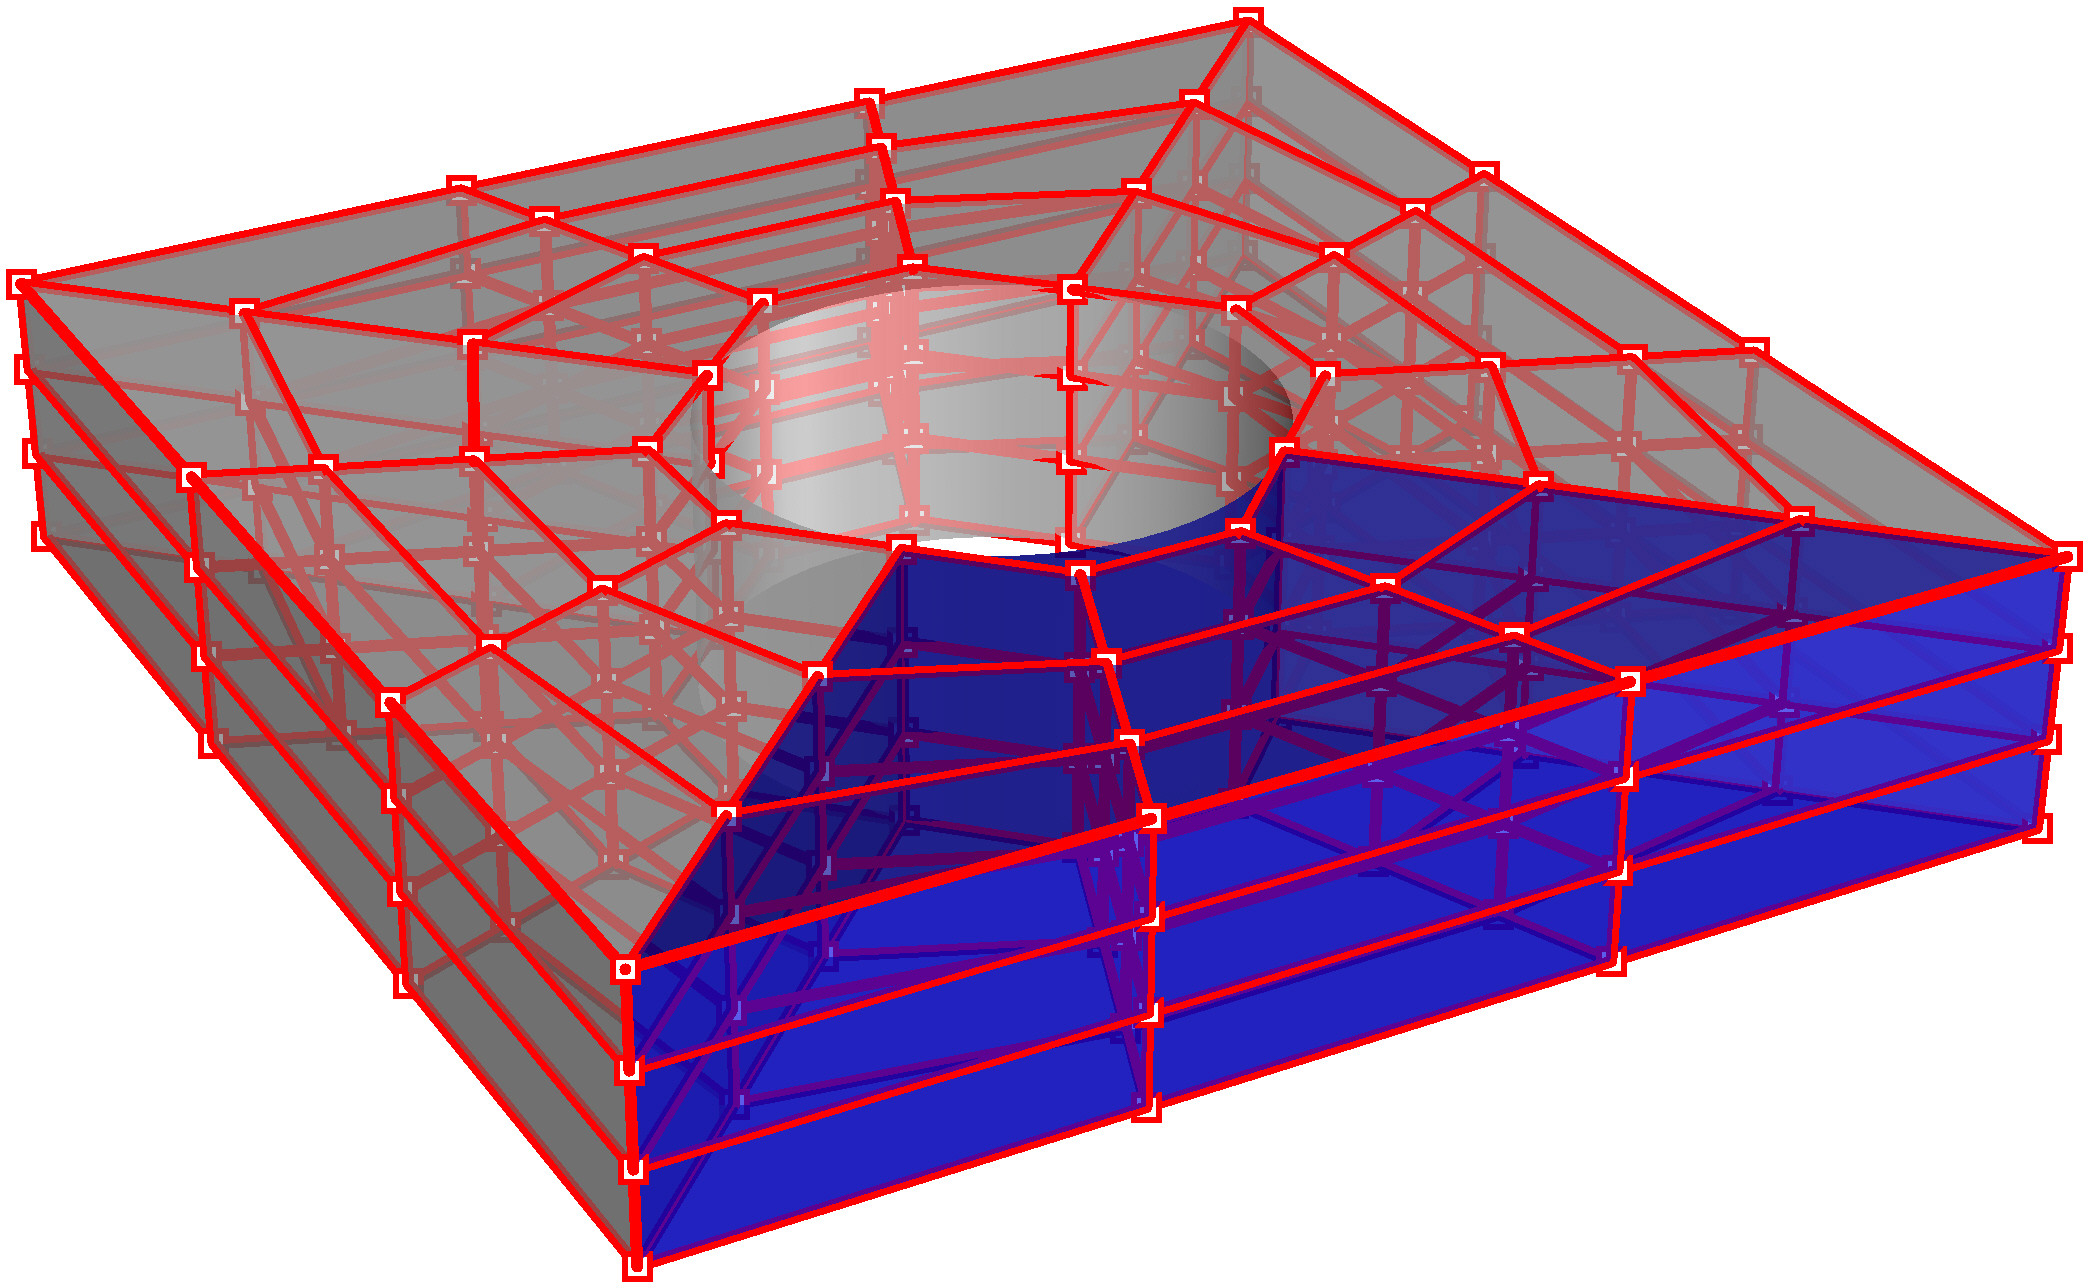
\includegraphics[height=2.55cm]{figures/CAD_07.jpg}
  \end{center}

  \begin{itemize}
    \item Opérations booléennes et géométries trimmées
  \end{itemize}
  \begin{center}
    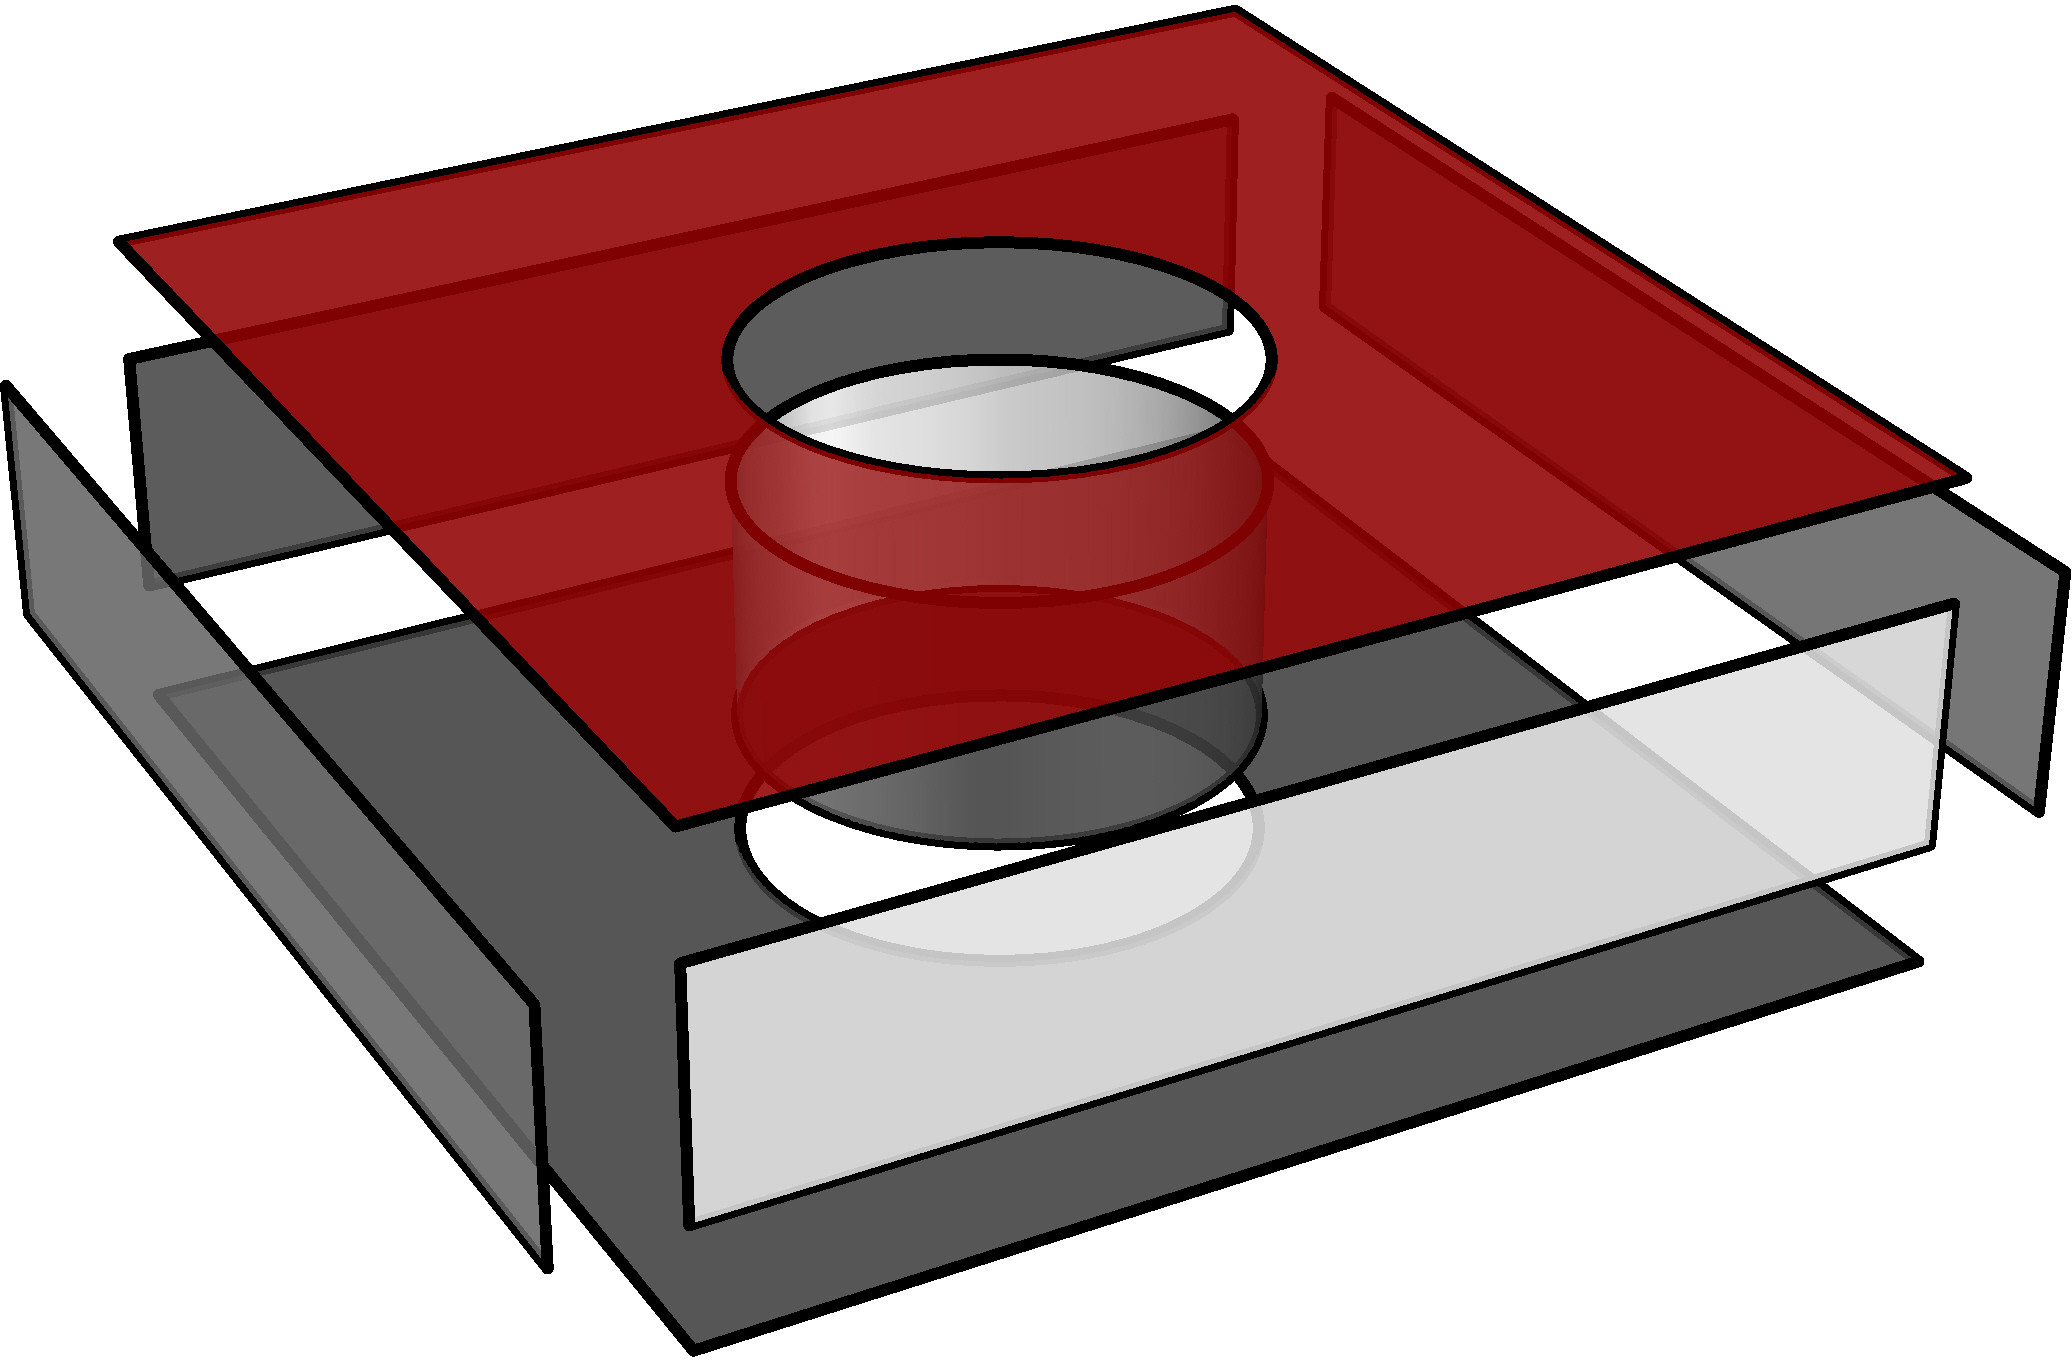
\includegraphics[height=2.5cm]{figures/CAD_03.jpg}
    \hspace{1cm}
    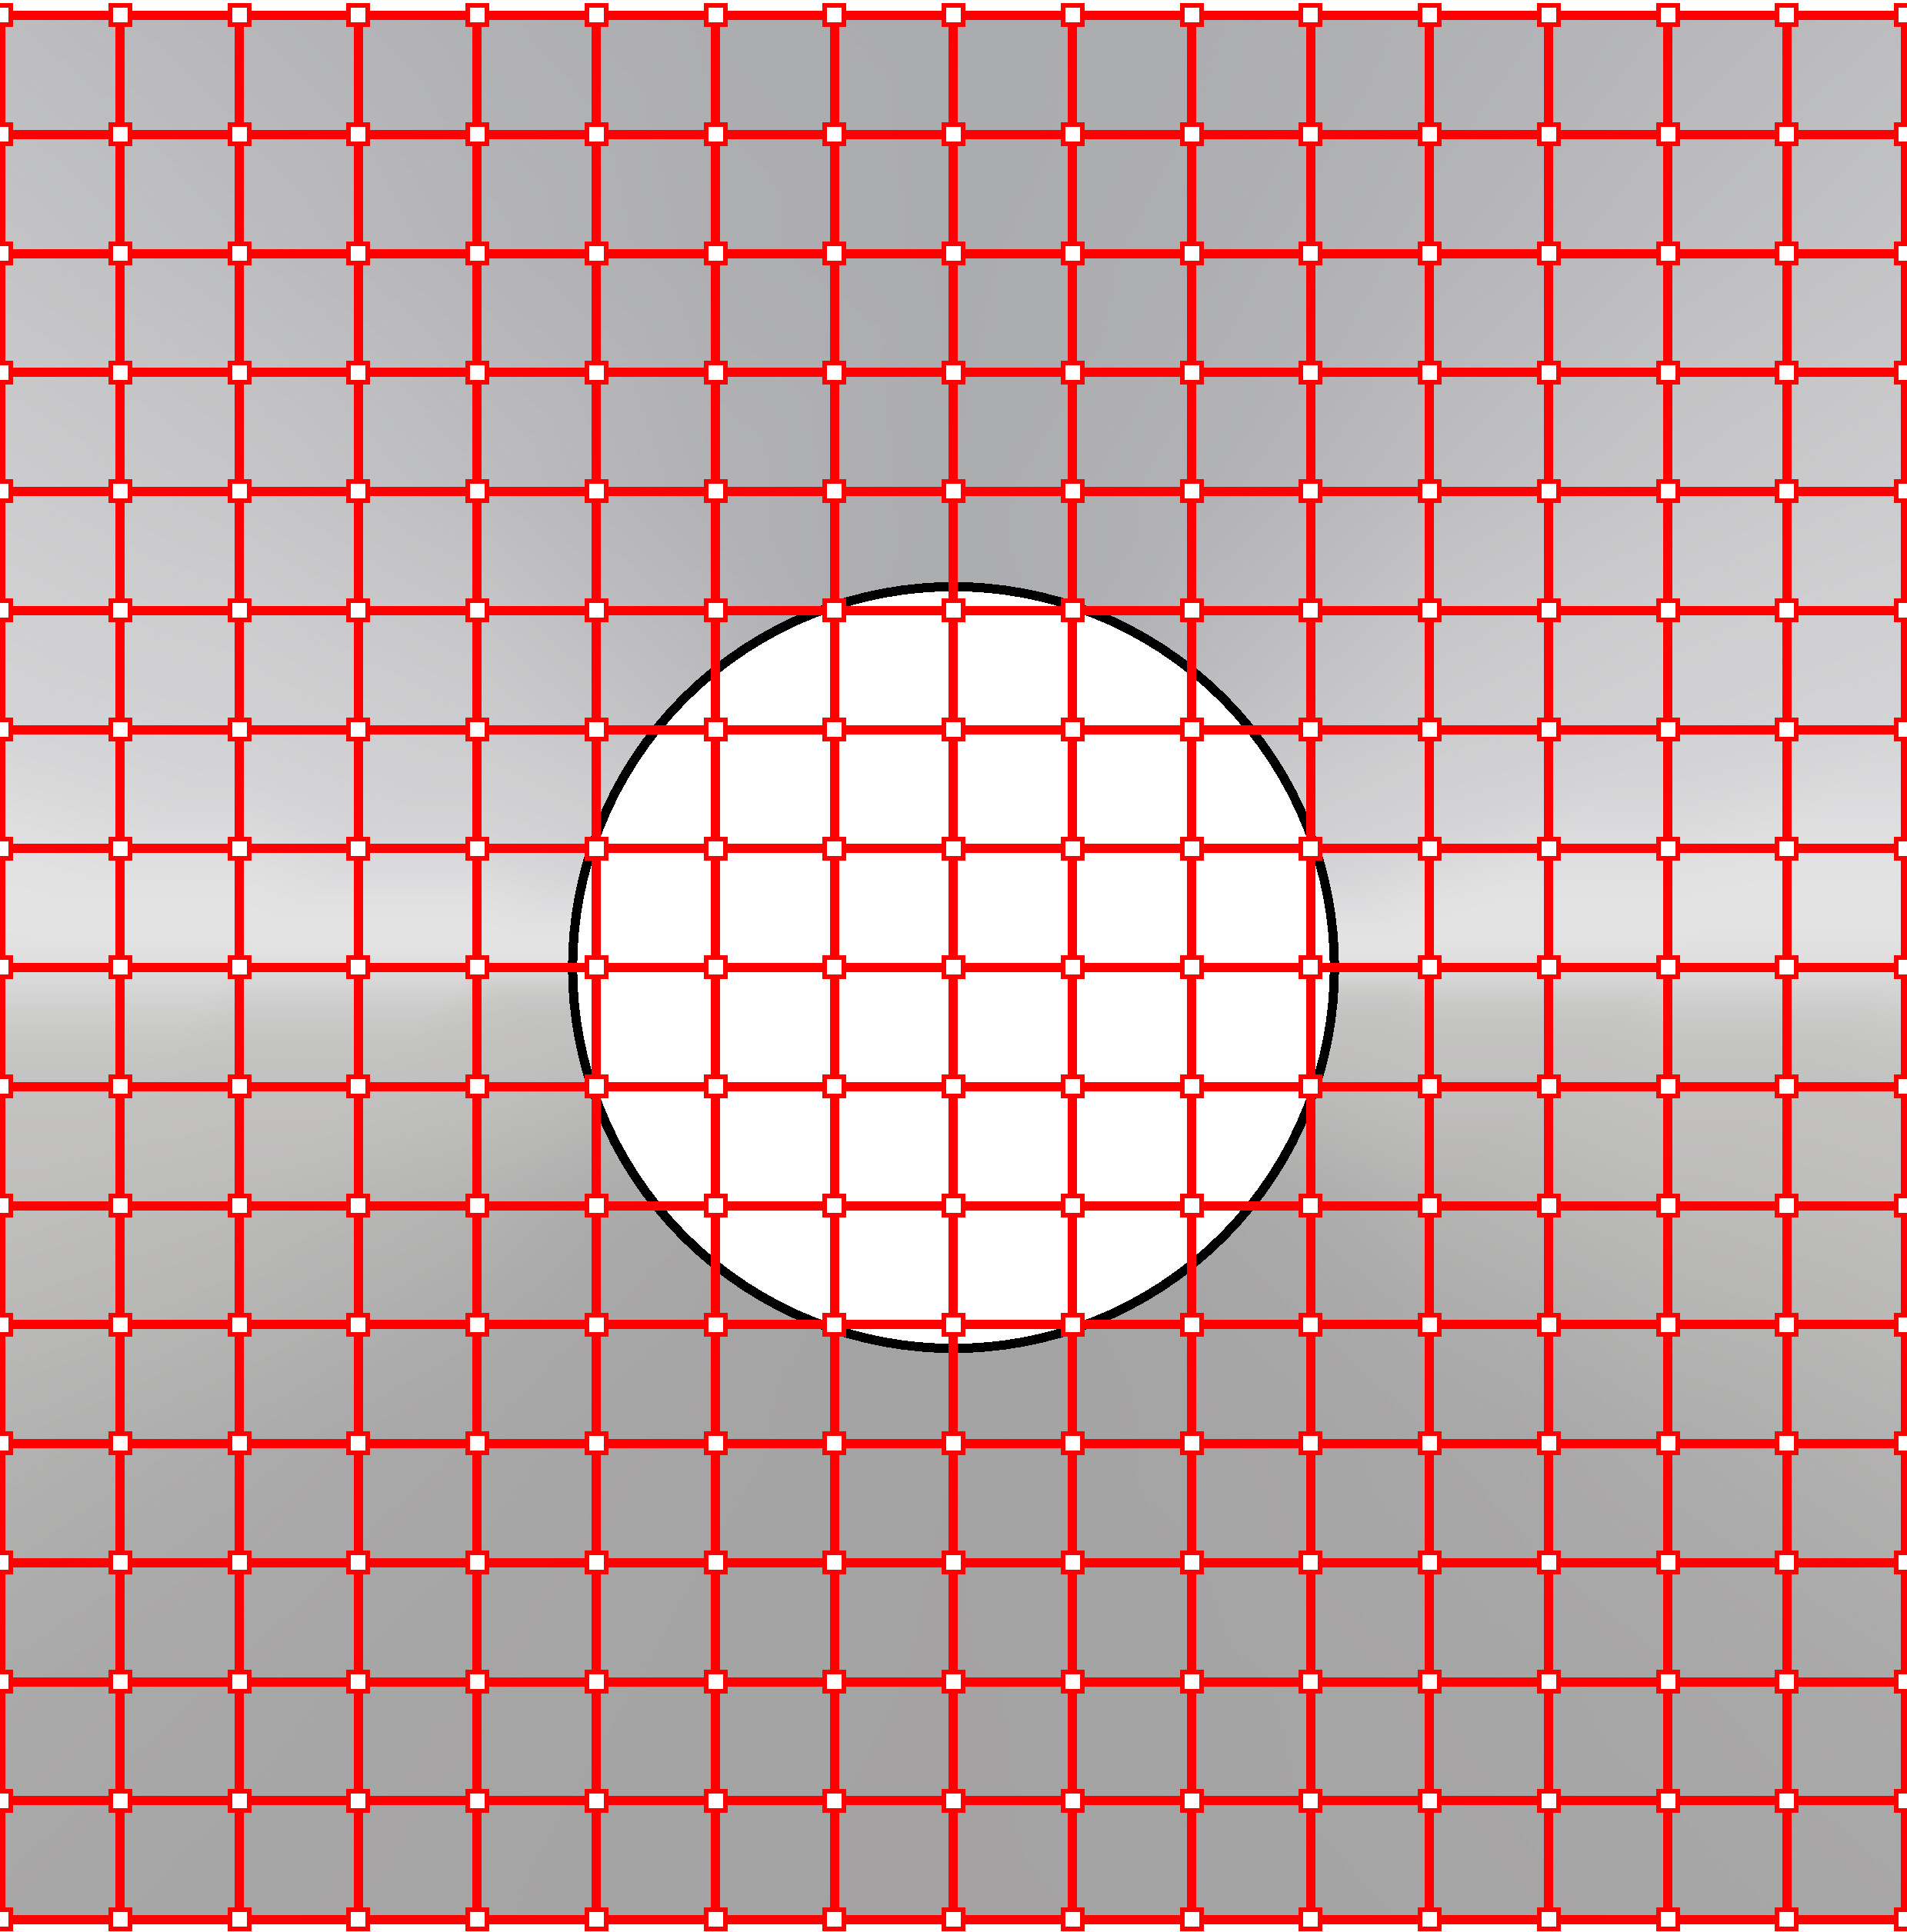
\includegraphics[height=2.5cm]{figures/CAD_05.jpg}
    \hspace{1cm}
    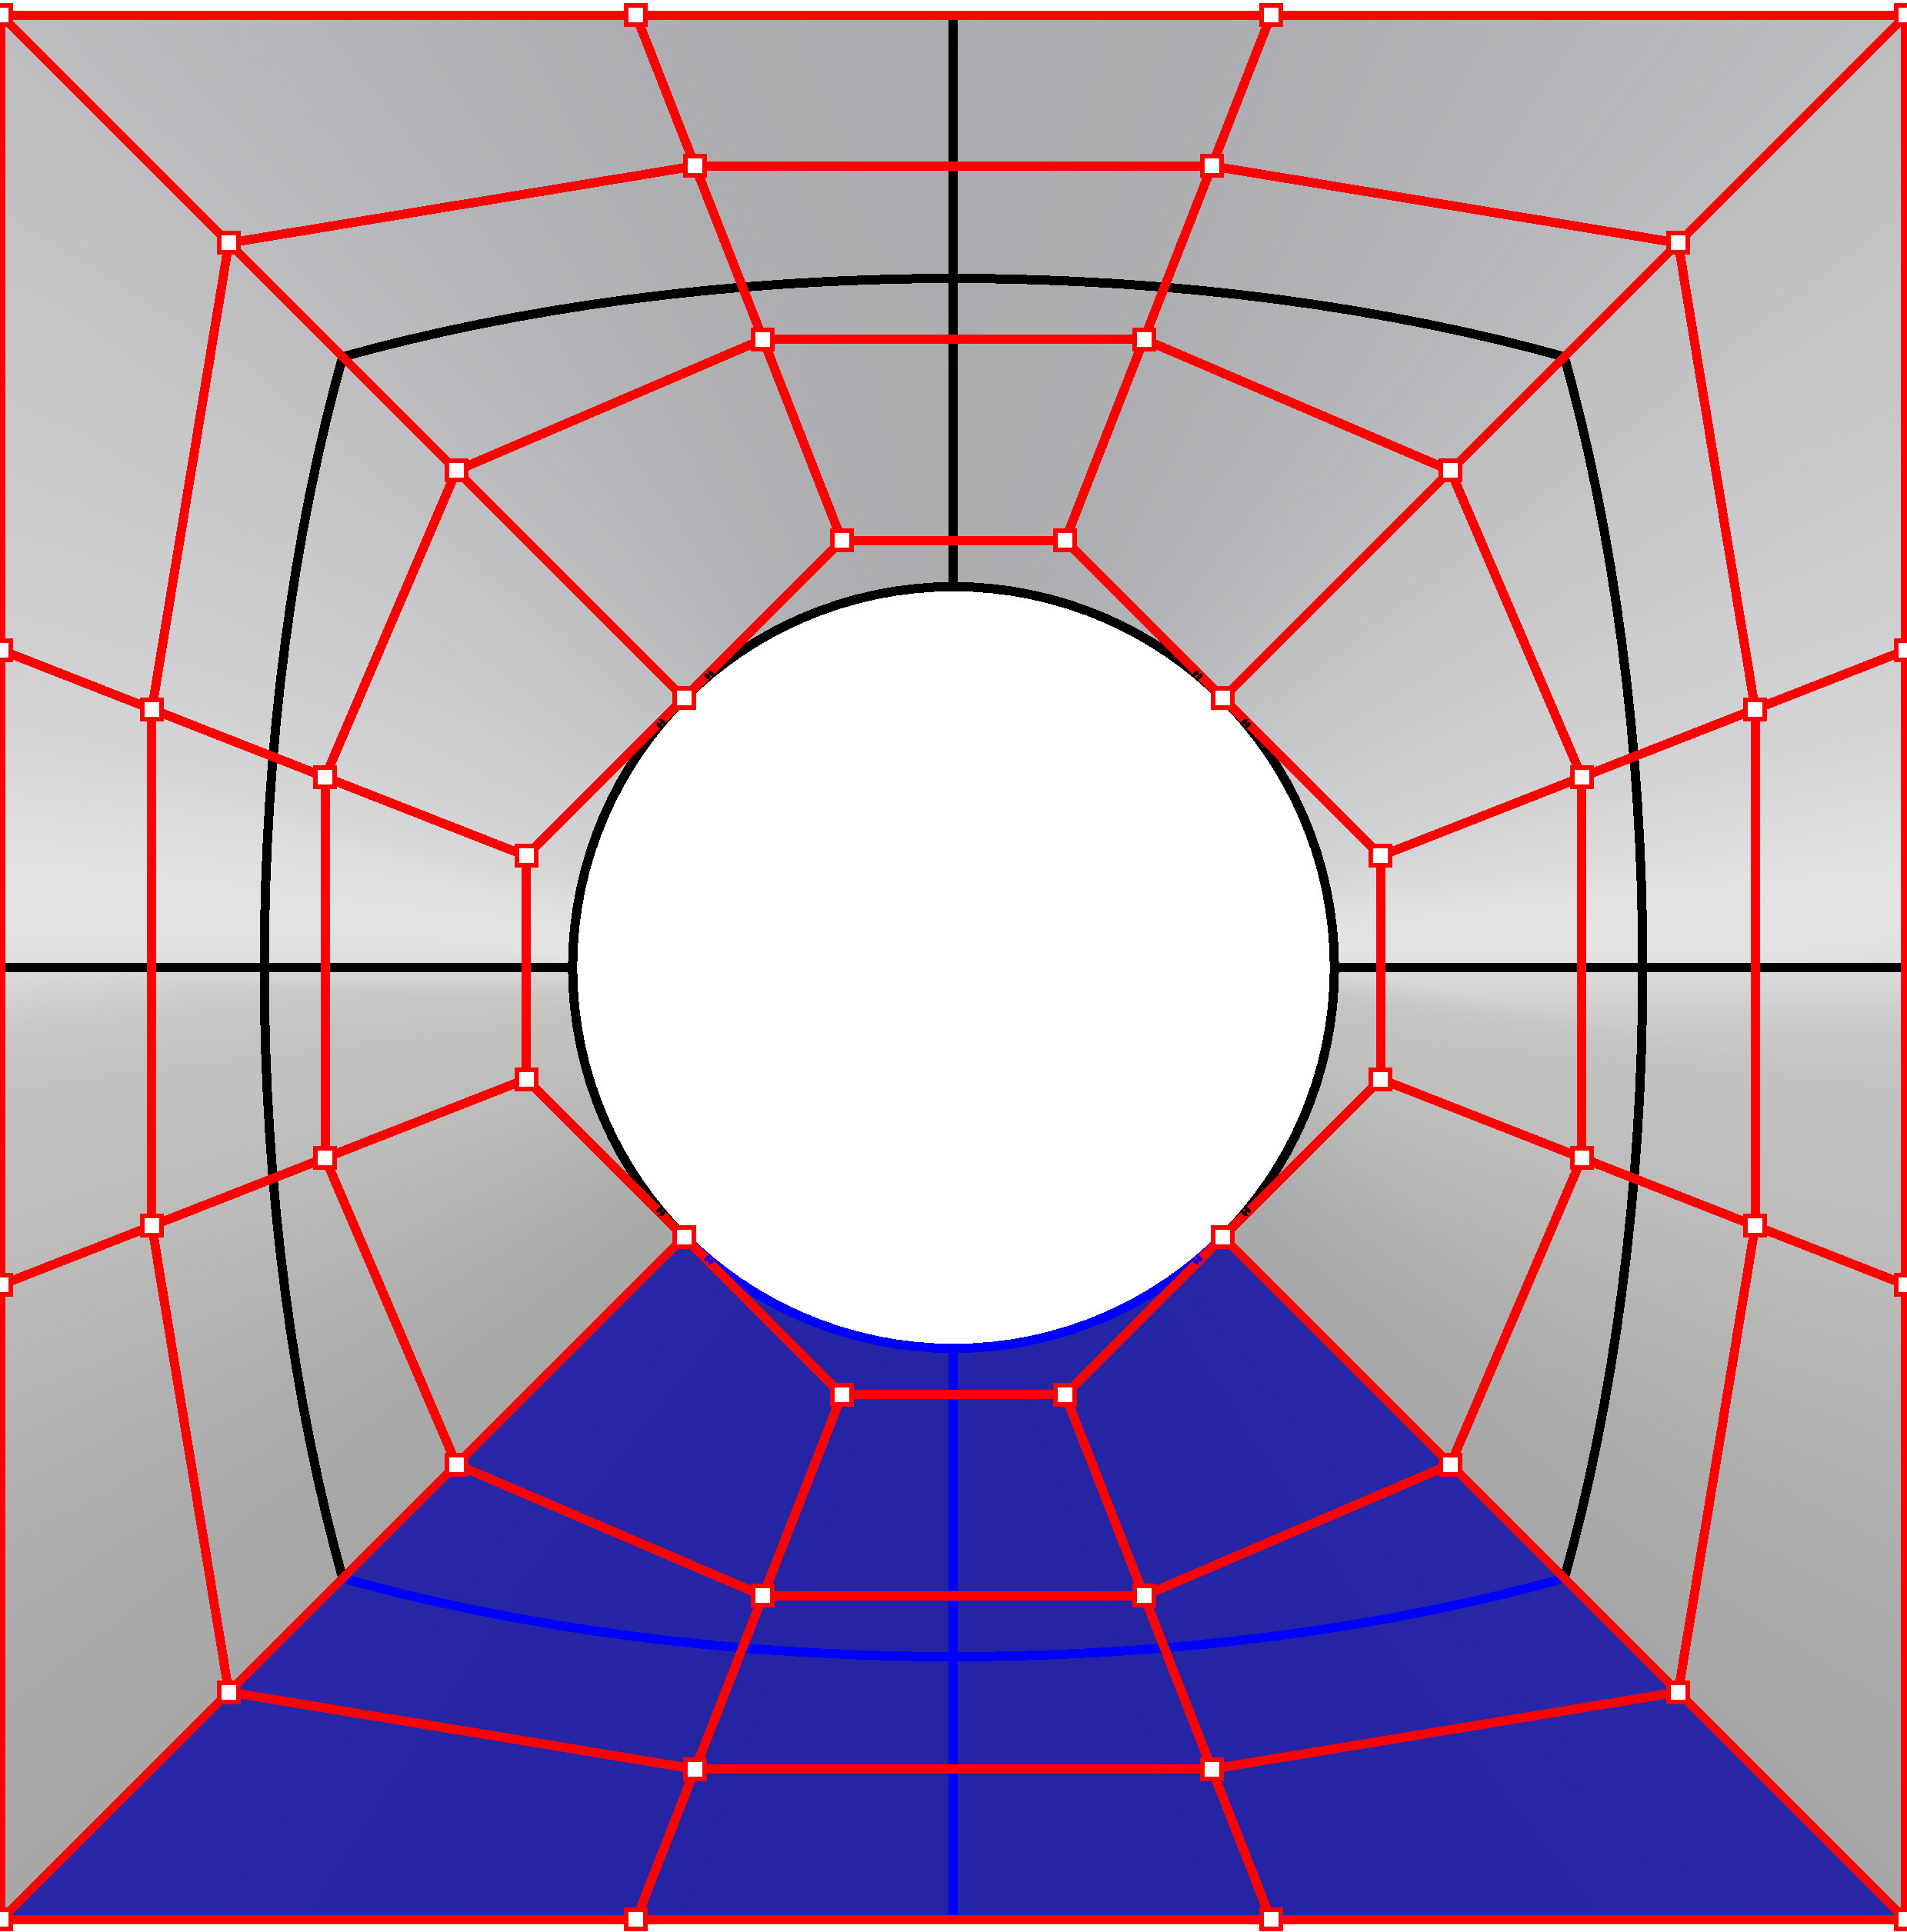
\includegraphics[height=2.5cm]{figures/CAD_06.jpg}
  \end{center}
\end{frame}

\begin{frame}
  \frametitle{Modélisation NURBS}
  \begin{itemize}
    \item On ne considère ici que les B-splines et les NURBS
    \item Représentation des objets géométriques sous forme {\bf paramétrique}
  \end{itemize}
  \begin{columns}
    \begin{column}{0.65 \linewidth}
      \begin{itemize}
        \item Exemple d'une courbe dans un plan
        \begin{itemize}
          \item Expression générale
          \begin{equation*}
            C(\xi) = \left( x(\xi), y(\xi) \right) \quad \forall \xi \in \mathcal{U}
          \end{equation*}
          \item B-splines et NURBS
          \begin{equation*}
            C(\xi) = \sum_{i=1}^{n} N_i(\xi) P_i \quad \forall \xi \in [0, 1]
          \end{equation*}
          \begin{itemize}
            \item B-splines : $N_i$ polynômes
            \item NURBS : $N_i$ fractions rationnelles de polynômes
          \end{itemize}
        \end{itemize}
      \end{itemize}
    \end{column}
    \begin{column}{0.35\linewidth}
      \begin{center}
        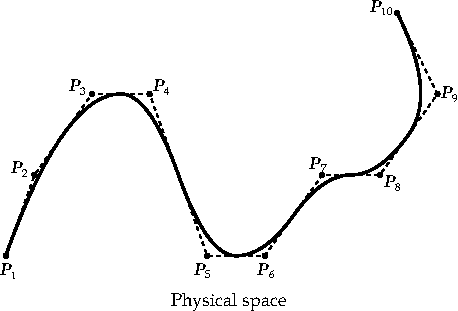
\includegraphics[width=0.9\linewidth]{figures/9_bsplineExample-1.pdf}
        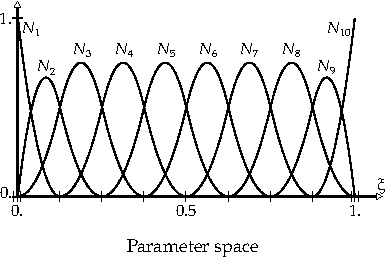
\includegraphics[width=0.8\linewidth]{figures/9_bsplineExample-2.pdf}
      \end{center}
    \end{column}
  \end{columns}
\end{frame}

\begin{frame}
  \frametitle{Surface et volumes}
  \begin{itemize}
    \item Construction des fonctions de forme par {\bf produit tensoriel}
    \vspace{0.2cm}
    \begin{center}
      \only<1>{
          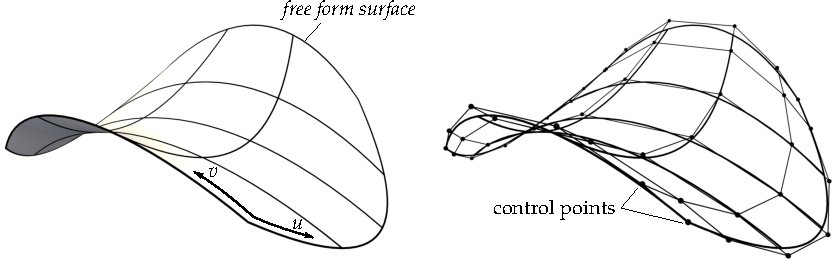
\includegraphics[width=0.7\linewidth]{figures/15_surfaceExamples.pdf}
          \begin{equation*}
            S(\xi, \eta) = \sum_{i=1}^{n_\xi} \sum_{j=1}^{n_\eta} N_{ij} (\xi, \eta) P_{ij}
          \end{equation*}
          \begin{equation*}
            N_{ij}(\xi, \eta) = N_i(\xi) M_j(\eta)
          \end{equation*}
      }
      \only<2>{
          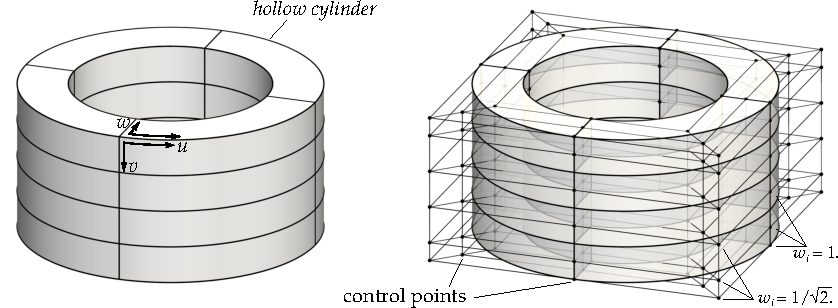
\includegraphics[width=0.7\linewidth]{figures/16_volumeExamples.pdf}
          \begin{equation*}
            V(\xi, \eta, \zeta) = \sum_{i=1}^{n_\xi} \sum_{j=1}^{n_\eta} \sum_{k=1}^{n_\zeta} N_{ijk} (\xi, \eta, \zeta) P_{ijk}
          \end{equation*}
          \begin{equation*}
            N_{ijk}(\xi, \eta, \zeta) = N_i(\xi) M_j(\eta) L_k(\zeta)
          \end{equation*}
      }
    \end{center}
  \end{itemize}
\end{frame}

\begin{frame}
  \frametitle{Fonctions de forme B-Spline : construction \cite{piegl_nurbs_1997}}
  \begin{itemize}
    \item {\bf Vecteur de n\oe{}uds} (\emph{knot vector}) : ensemble de coordonnées dans l'espace paramétrique
    \begin{equation}
      \Xi = \left\{ \xi_1, \dots, \xi_{n+p+1} \right\}
    \end{equation}
    \item Un intervalle (\emph{span}) $\equiv$ un élément
    \item Construction récursive des $n$ fonctions de degré $p$, $N_{i, p}$ (formule de Cox-DeBoor) pour un \emph{knot vector} $\Xi$
    \only<1>{
      \begin{equation*}
        N_{i, 0} (\xi)= \left\{
          \begin{array}{ll}
            1 & \textrm{si} \quad \xi_i \le \xi < \xi_{i+1} \\
            0 & \textrm{sinon}
          \end{array}\right.
      \end{equation*}
      \begin{equation*}
        N_{i,p} (\xi) = \frac{\xi - \xi_i}{\xi_{i+p} - \xi_i} N_{i, p-1} (\xi) + \frac{\xi_{i+p+1} - \xi}{\xi_{i+p+1} - \xi_{i+1}} N_{i+1, p-1} (\xi)
      \end{equation*}
    }
    \only<2>{
      \begin{center}
        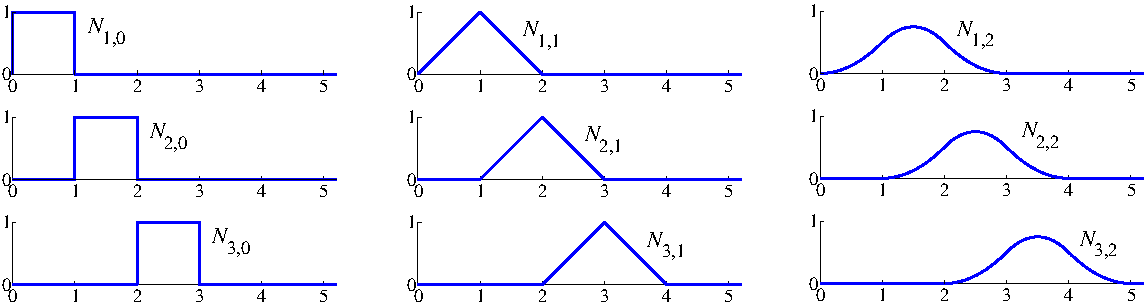
\includegraphics[width=.9\linewidth]{figures/basis_funs_roman.pdf}
      \end{center}
    }
  \end{itemize}
\end{frame}

\begin{frame}
  \frametitle{Fonctions de forme B-Spline : continuité}
  \only<1>{
    \begin{itemize}
      \item La multiplicité d'un \emph{knot} modifie la régularité des fonctions B-Spline en ce point du domaine paramétrique :\\
      $N_{i,p}$ est de classe $\mathcal{C}^{p-{m_i}}$ au n\oe{}ud $\xi_i$ de multiplicité $m_i$
      \item Exemple de base quadratique $\mathcal{C}^1 / \mathcal{C}^0$ ($p=2$) pour le \emph{knot vector} ouvert non-uniforme
      \begin{equation*}
        \Xi = \left\{ {\color{red} 0, 0, 0}, 1, 2, 3, {\color{blue} 4, 4}, {\color{red}5, 5, 5} \right\}
      \end{equation*}
    \end{itemize}
  }
  \begin{center}
    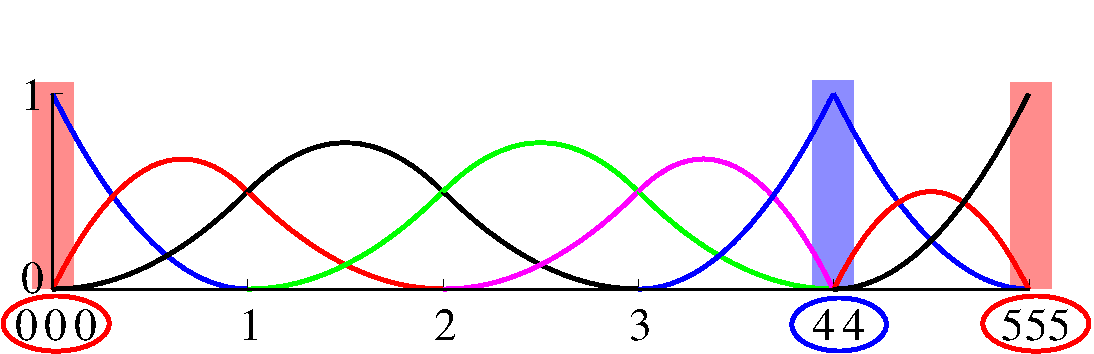
\includegraphics[width=0.6\linewidth]{figures/bspline_1d_23.pdf}\\
    \only<2>{
      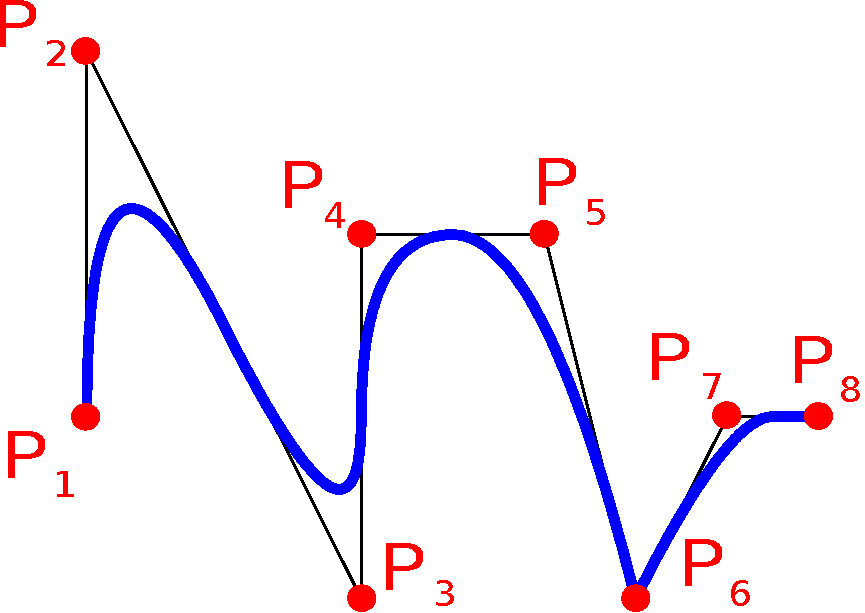
\includegraphics[width=0.3\linewidth]{figures/bspline_mesh.pdf}
      \hspace{1cm}
      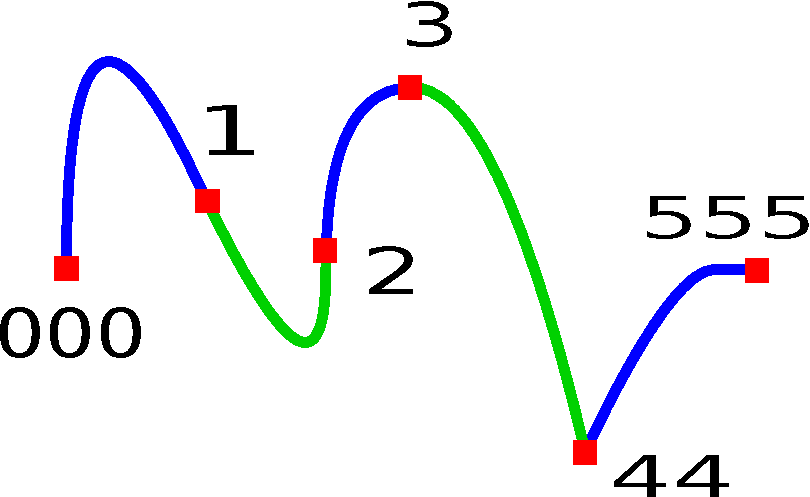
\includegraphics[width=0.3\linewidth]{figures/bspline_curve.pdf}
    }
  \end{center}
\end{frame}

\begin{frame}
  \frametitle{Raffinements $h$ et $p$}
  \begin{itemize}
    \item Insertion de nouveaux \emph{knots} (sans changer la courbe) : raffinement $h$
    \item Augmentation du degré polynomial (ou élévation d'ordre) des fonctions (sans changer la courbe) : raffinement $p$
  \end{itemize}
  \begin{center}
    \resizebox{0.7\linewidth}{!}{\input{figures/h_and_p_ref.pdf_t}}
  \end{center}
\end{frame}

\begin{frame}
  \frametitle{Raffinement $k$}
  \begin{itemize}
      \item Élévation d'ordre (raffinement $p$) {\bf puis} insertion de \emph{knot} (raffinement h): produit moins de fonction que $h$ puis $p$ avec une continuité supérieure
  \end{itemize}
  \begin{center}
    \resizebox{0.7\linewidth}{!}{\input{figures/hp-ph-ref2.pdf_t}}
  \end{center}
\end{frame}


\section[IGA]{Analyse ISOgéométrique}

\begin{frame}
  \frametitle{NURBS et éléments finis}
  \begin{itemize}
    \item Les {\color{blue}surfaces} et les {\color{blue} solides} B-Spline ou NURBS sont définis à partir d'un {\color{red} filet de contrôle} et de \emph{knot vectors} $(\Xi, \mathcal{H}, \mathcal{Z})$
    \begin{equation*}
      {\color{blue} \mathcal{S}} (\xi, \eta, \zeta) = \sum_{i=1}^n \sum_{j=1}^m \sum_{k=1}^l N_{i, p} (\xi) M_{j, q} (\eta) L_{k, r} (\zeta) {\color{red} B_{ijk}}
    \end{equation*}
    \item $\Xi \times \mathcal{H} \times \mathcal{Z}$ définit un maillage dans l'espace paramétrique
  \end{itemize}
  \begin{center}
    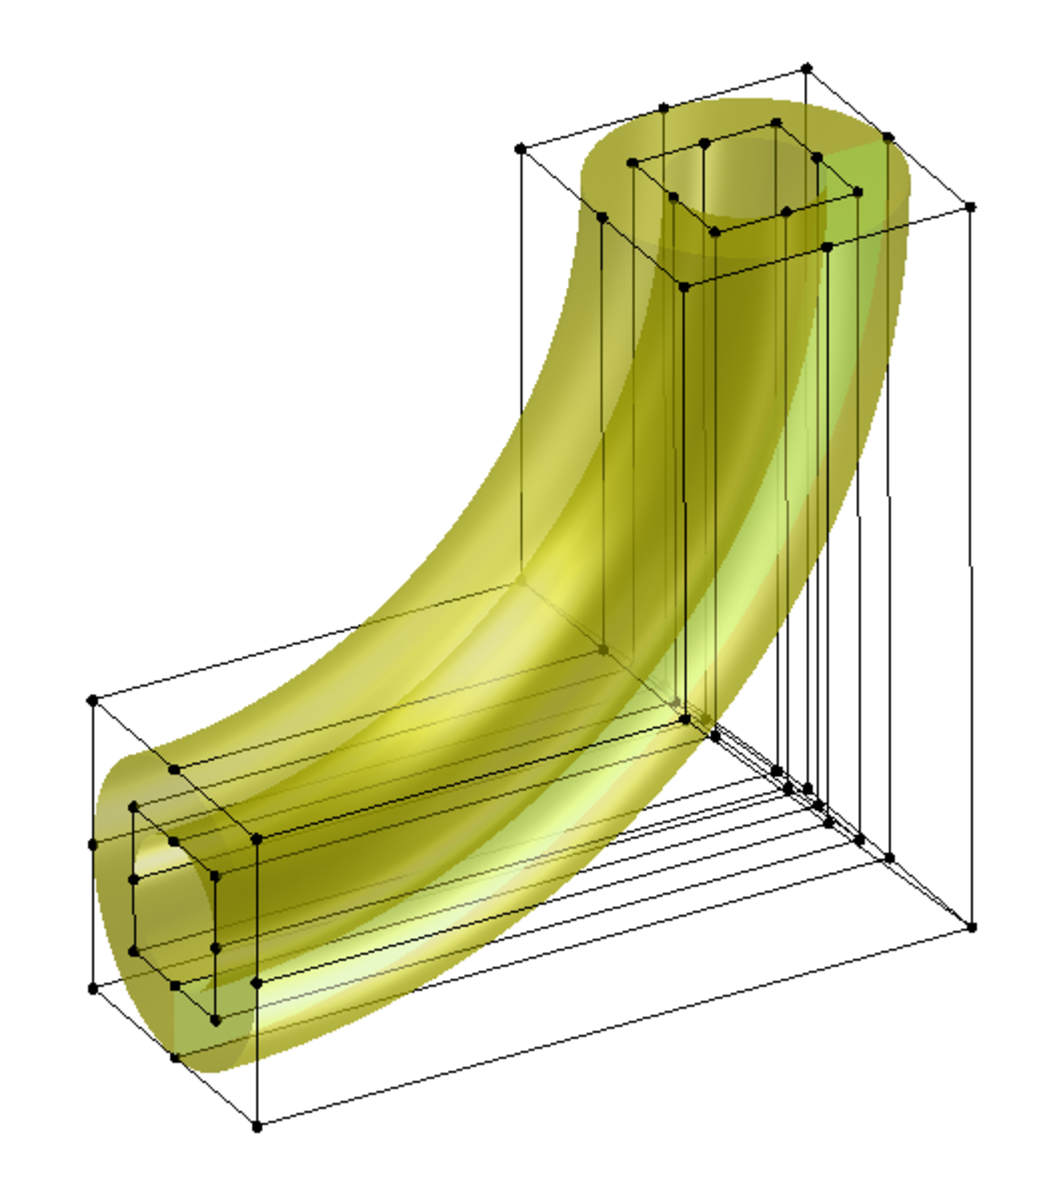
\includegraphics[width=0.24\linewidth]{figures/tube_geom_control_mesh.pdf}
    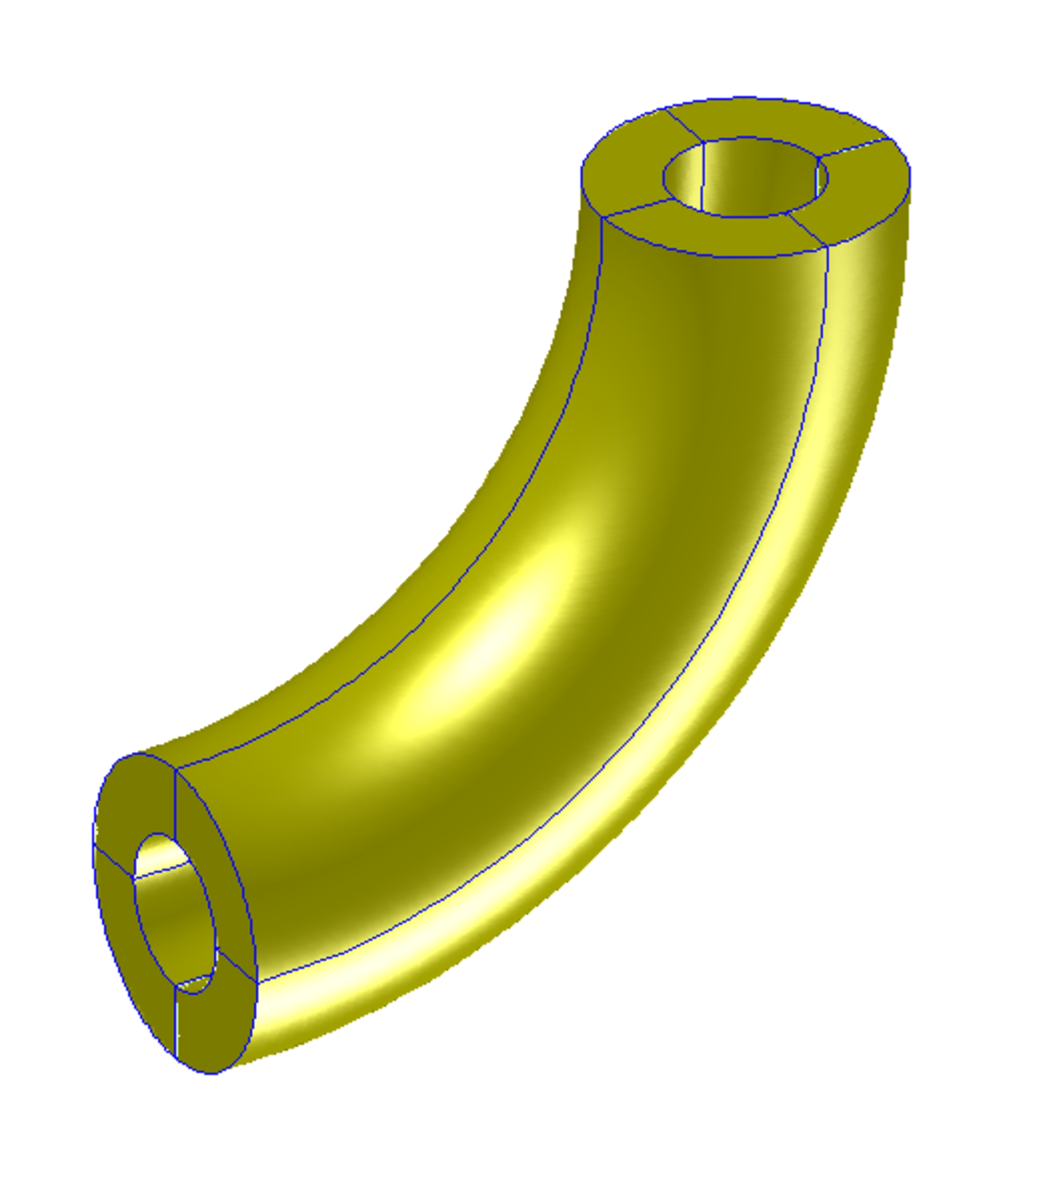
\includegraphics[width=0.24\linewidth]{figures/tube_geom.pdf}
    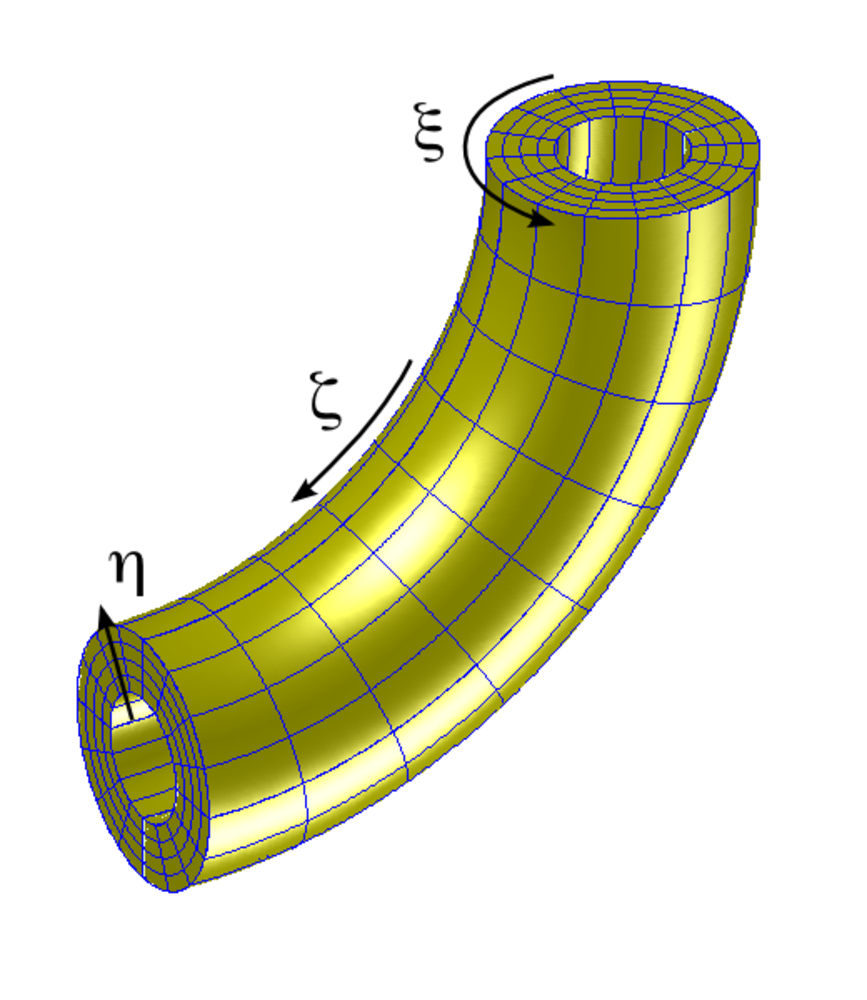
\includegraphics[width=0.24\linewidth]{figures/tube_mesh2.pdf}
  \end{center}
\end{frame}

\begin{frame}
  \frametitle{NURBS et éléments finis}
  \begin{itemize}
    \item Chaque point de contrôle est associé à une fonction de la base qui a pour support un petit nombre d'éléments
    \begin{equation*}
      {\color{blue} u} (\xi, \eta, \zeta) = \sum_{i=1}^n \sum_{j=1}^m \sum_{k=1}^l N_{i, p} (\xi) M_{j, q} (\eta) L_{k, r} (\zeta) {\color{red} U_{ijk}}
    \end{equation*}
  \end{itemize}
  \vspace{-1cm}
  \begin{columns}
    \begin{column}{0.5\linewidth}
      \begin{itemize}
        \item Le concept isoparamétrique est invoqué
        \item les coefficients de la base de fonction sont les {\bf variables de contrôle}
      \end{itemize}
    \end{column}
    \begin{column}{0.5\linewidth}
      \begin{center}
        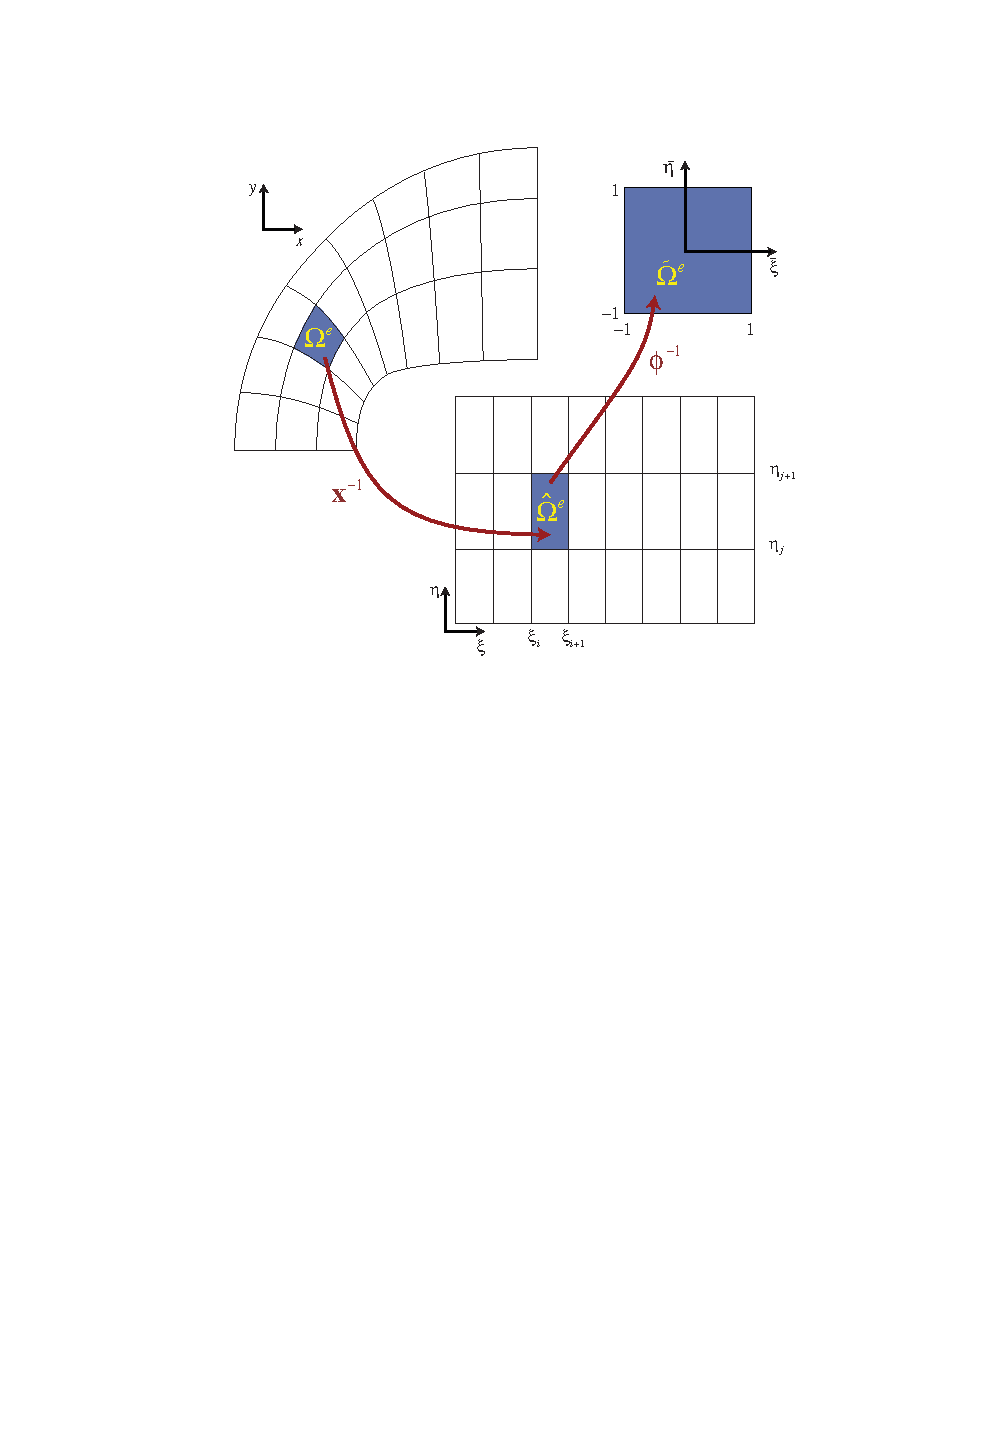
\includegraphics[width=0.8\linewidth]{figures/3repere.pdf}
      \end{center}
    \end{column}
  \end{columns}
\end{frame}

\begin{frame}
  \frametitle{Multipatch}
  \begin{itemize}
    \item Les formes simples peuvent être générées à partir d'un seul patch ("super élément")
    \item Les formes plus complexes sont souvent générées à partir d'assemblage de patchs
    \begin{center}
      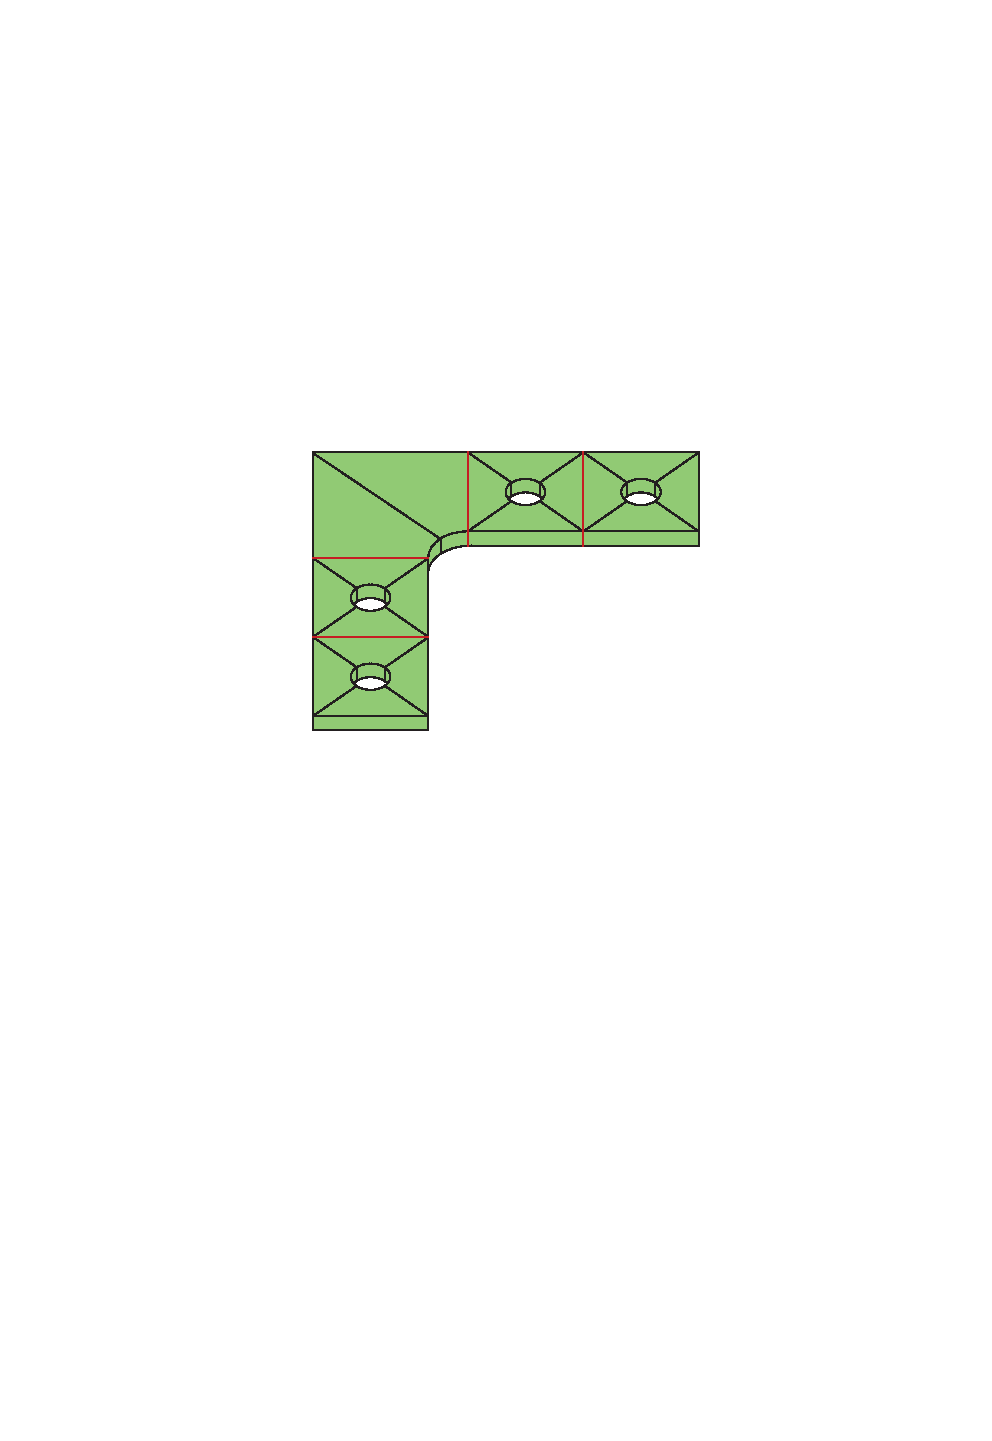
\includegraphics[width=0.3\linewidth]{figures/multipatch2.pdf}
      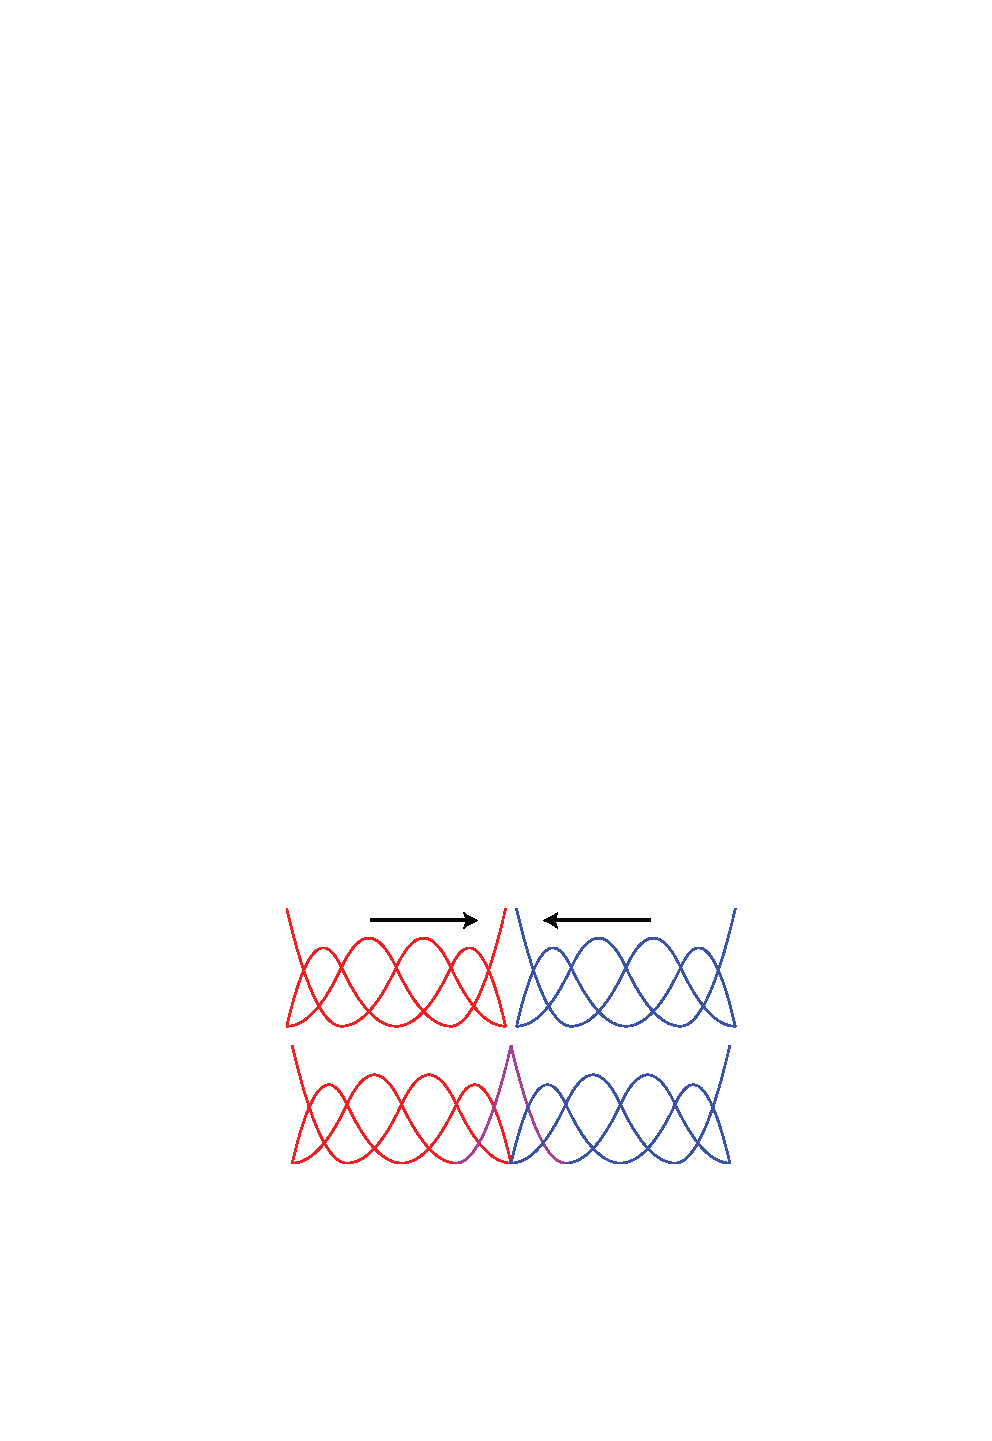
\includegraphics[width=0.4\linewidth]{figures/multipatch.pdf}
    \end{center}
    \item Raccord fort ou raccord faible
    \item Continuité dépendante de la géométrie : généralement $\mathcal{C}^0$ ou $\mathcal{G}^1$
  \end{itemize}
\end{frame}


\begin{frame}
  \frametitle{Implémentation - schéma général}
  \begin{center}
    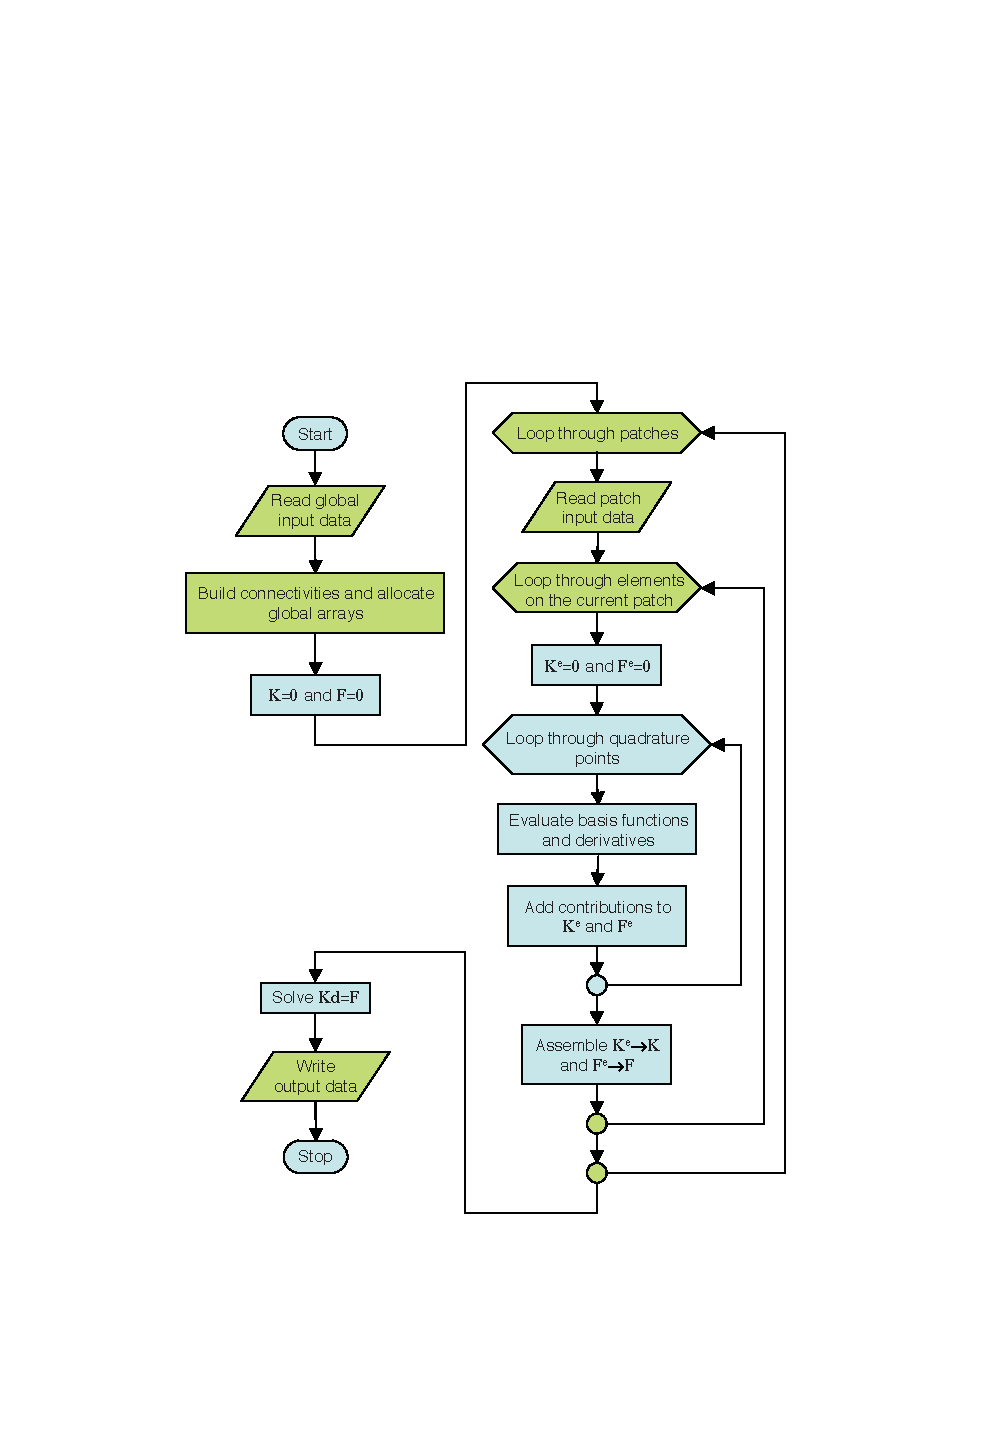
\includegraphics[width=0.35\linewidth]{figures/structure2.pdf}
  \end{center}
\end{frame}

\begin{frame}
  \frametitle{Implémentation - structure de données}
  \only<1-2>{
    \begin{center}
      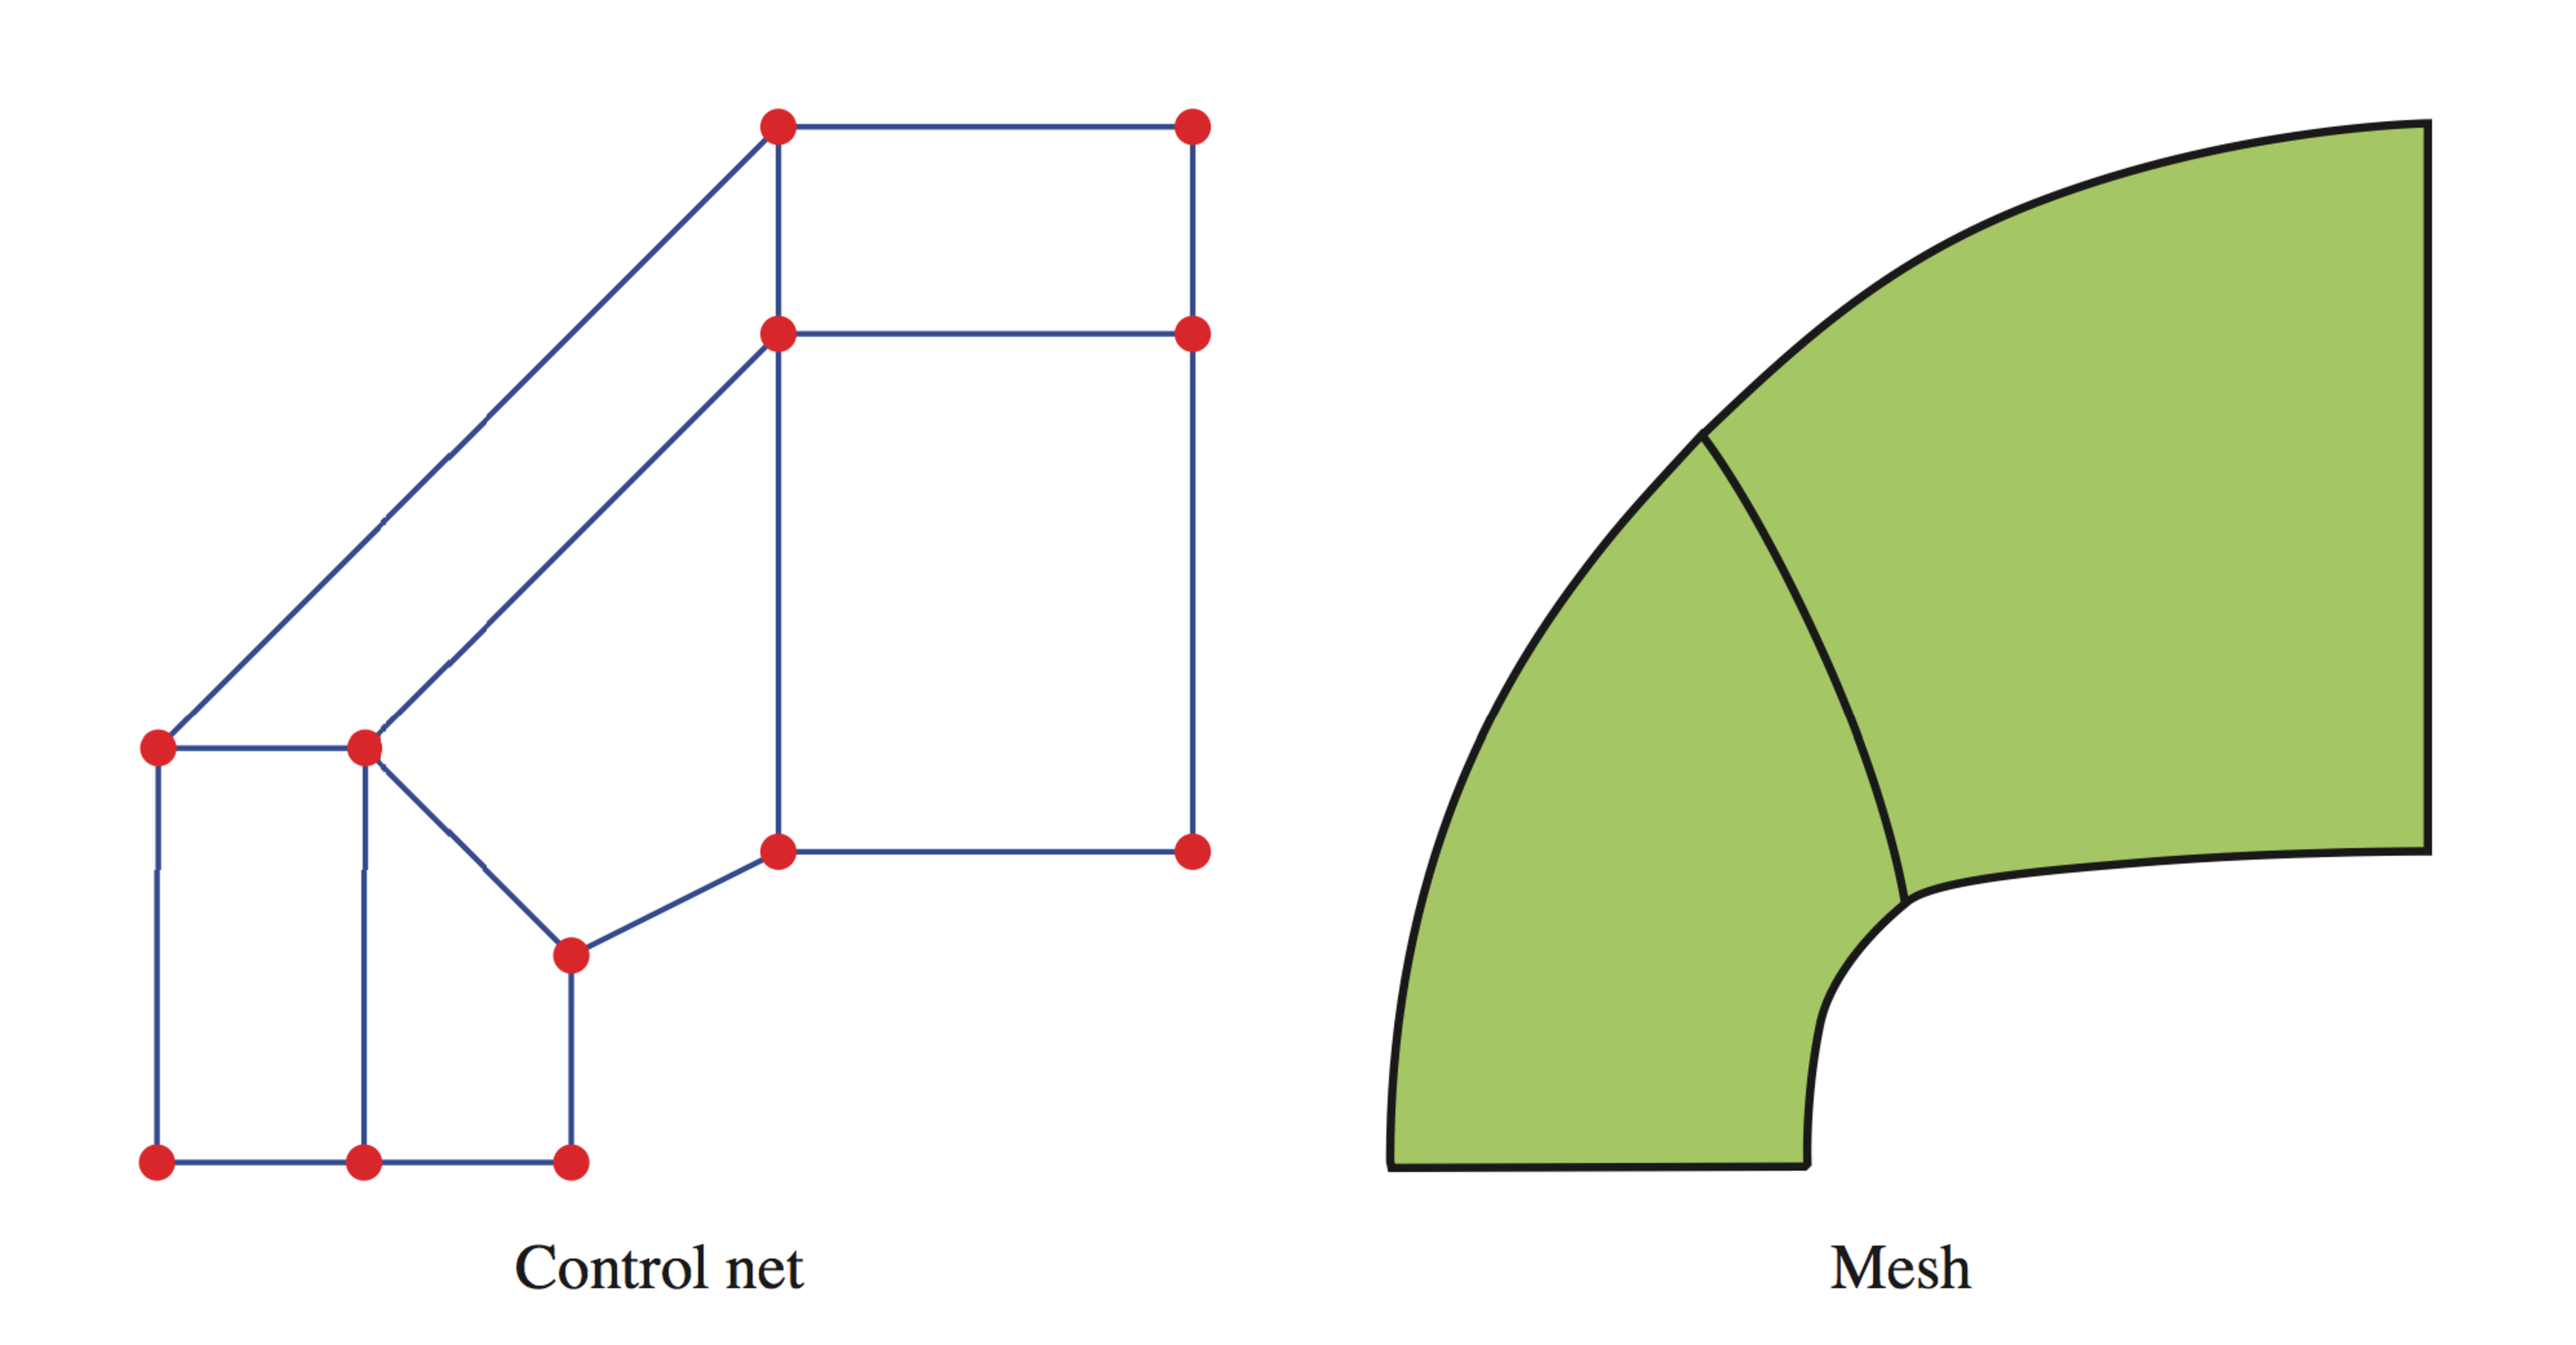
\includegraphics[width=0.4\linewidth]{figures/control_net.pdf} 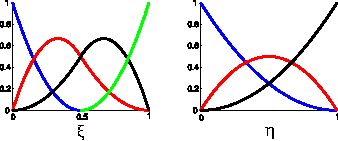
\includegraphics[width=0.45\linewidth]{figures/xi_eta.pdf}
    \end{center}
  }
  \only<1>{
    \begin{equation*}
      \Xi = \left\{ 0, 0, 0, 0.5, 1, 1, 1 \right\} \quad \mathcal{H} = \left\{ 0, 0, 0, 1, 1, 1 \right\}
    \end{equation*}
  }
  \only<3->{
    \begin{itemize}
      \item Élément 2
      \begin{itemize}
        \item \texttt{degrees : [2, 2]}
        \item \texttt{connectivity: [12, 11, 10, 8, 7, 6, 4, 3, 2]}
        \item \texttt{spans: [4, 3]}
      \end{itemize}
    \end{itemize}
  }
  \only<2->{
    \begin{center}
      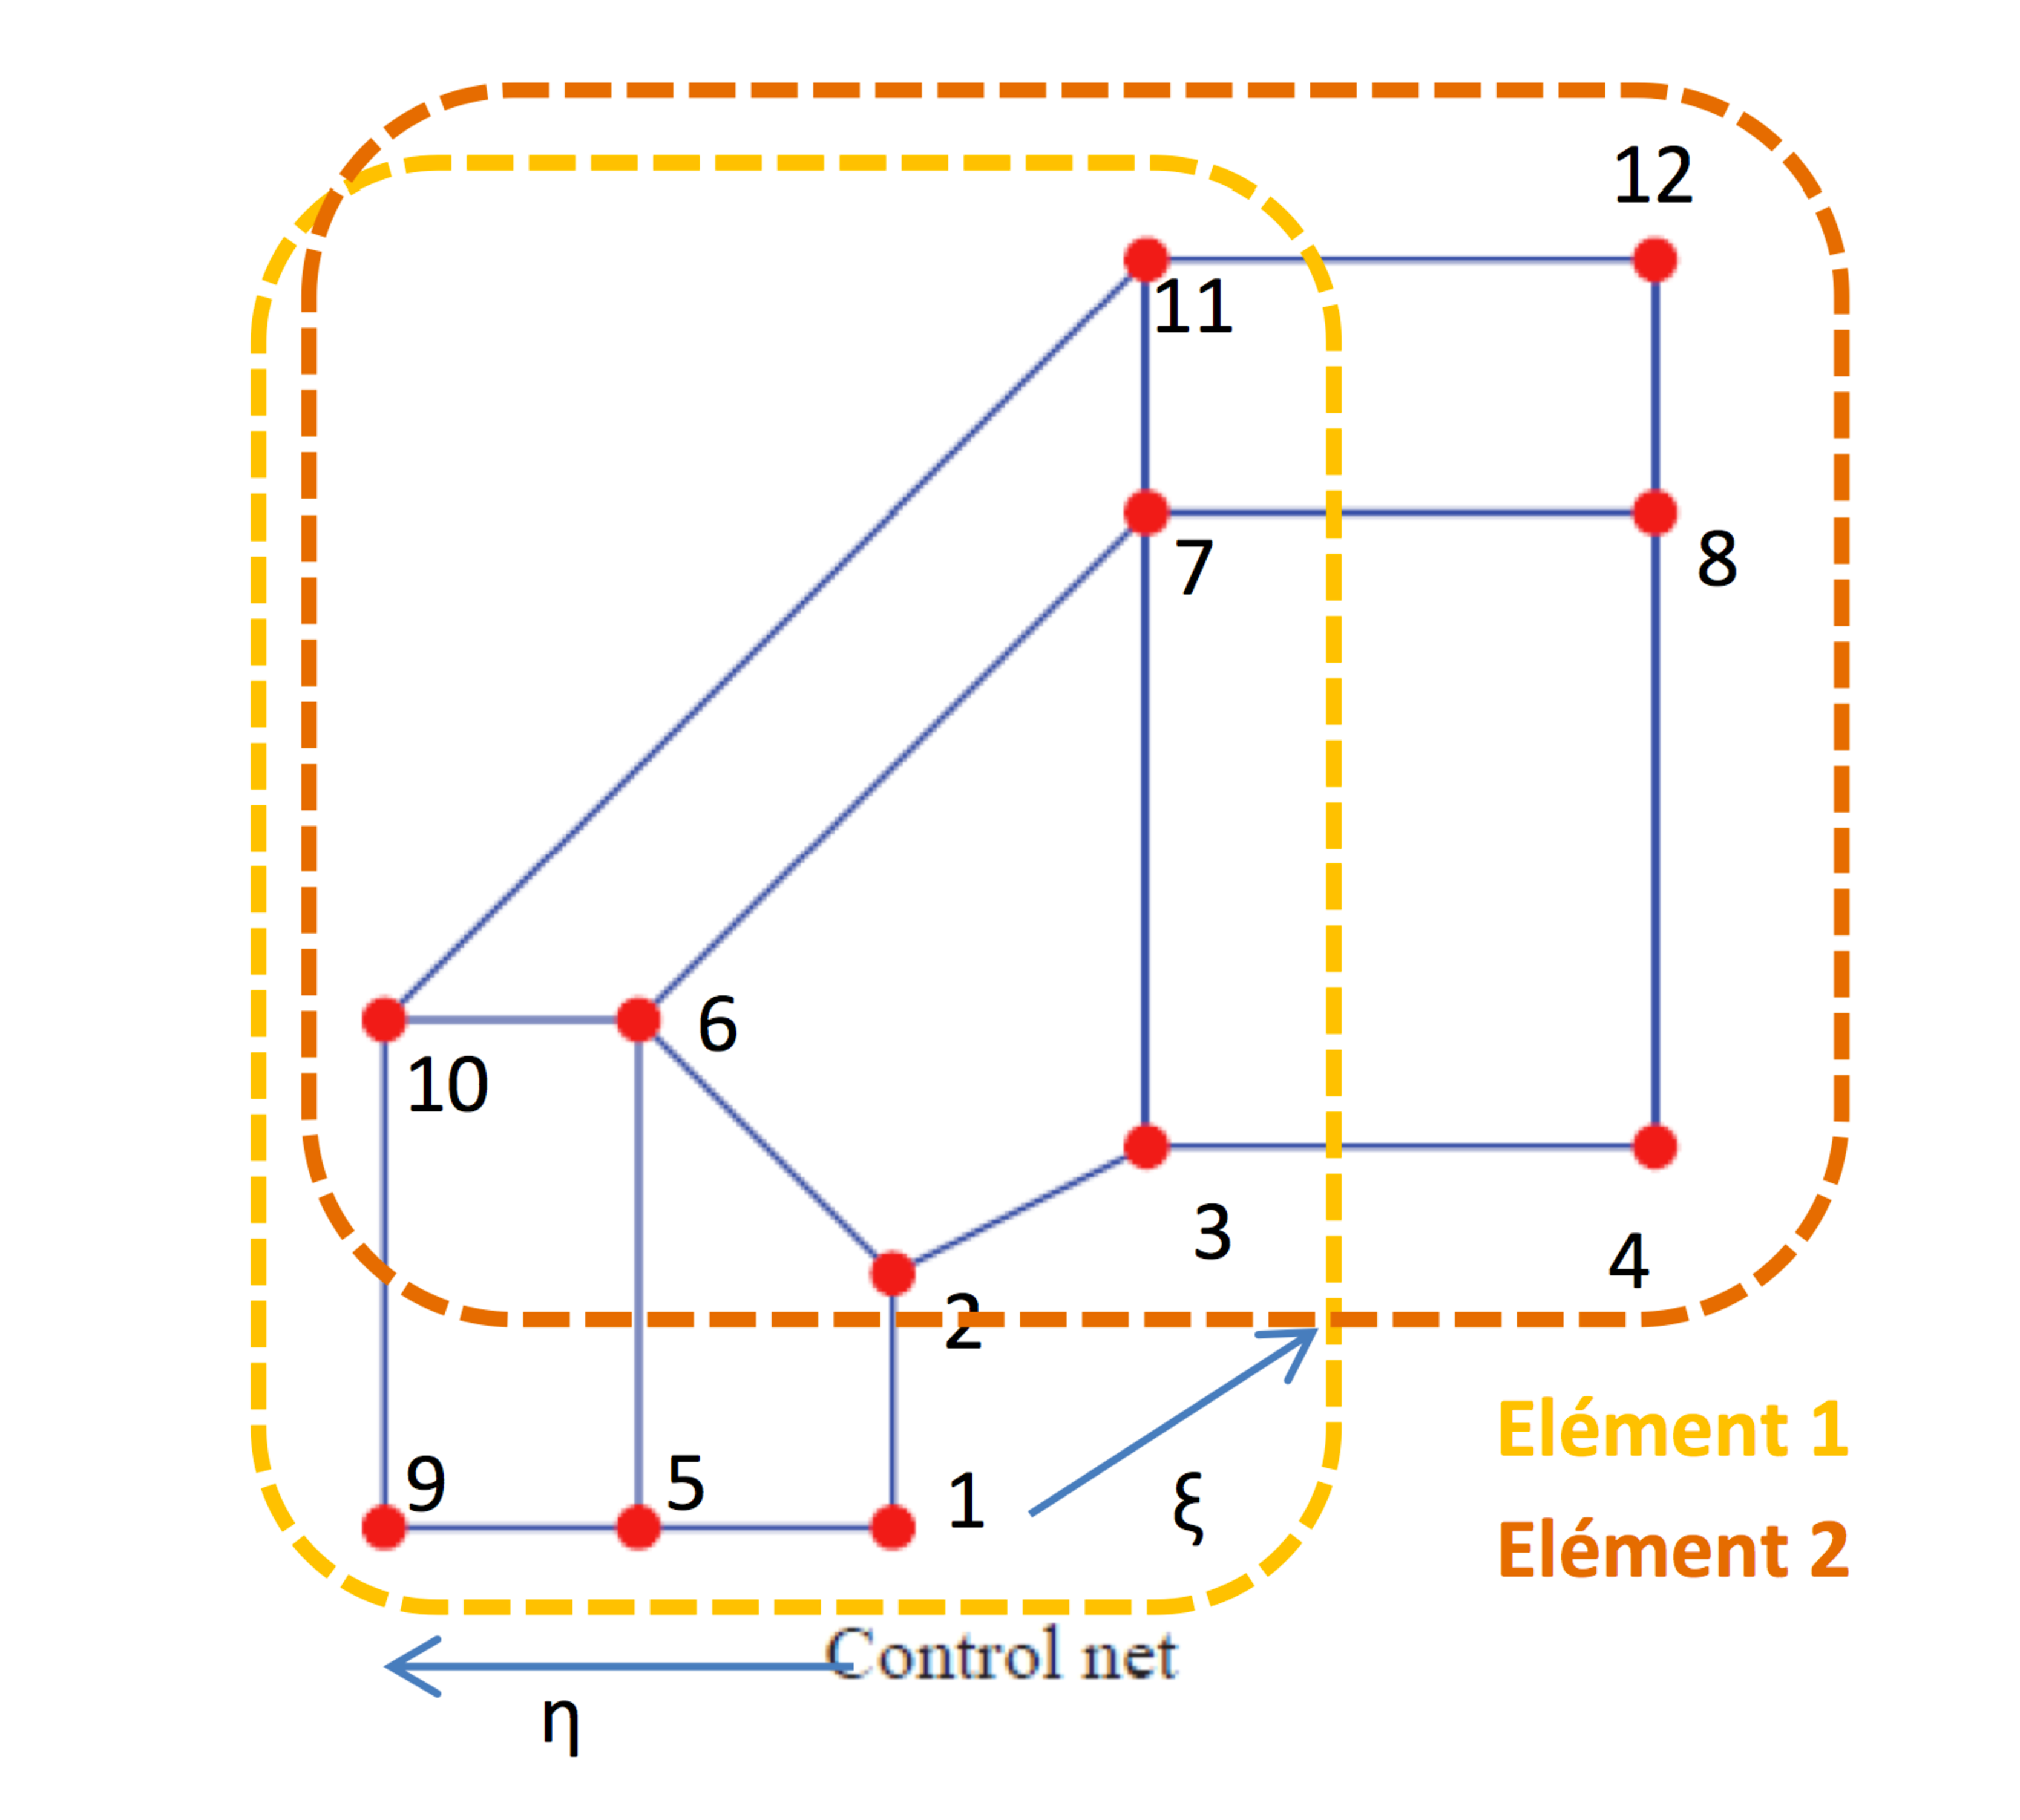
\includegraphics[width=0.28\linewidth]{figures/elem_conn.pdf}
      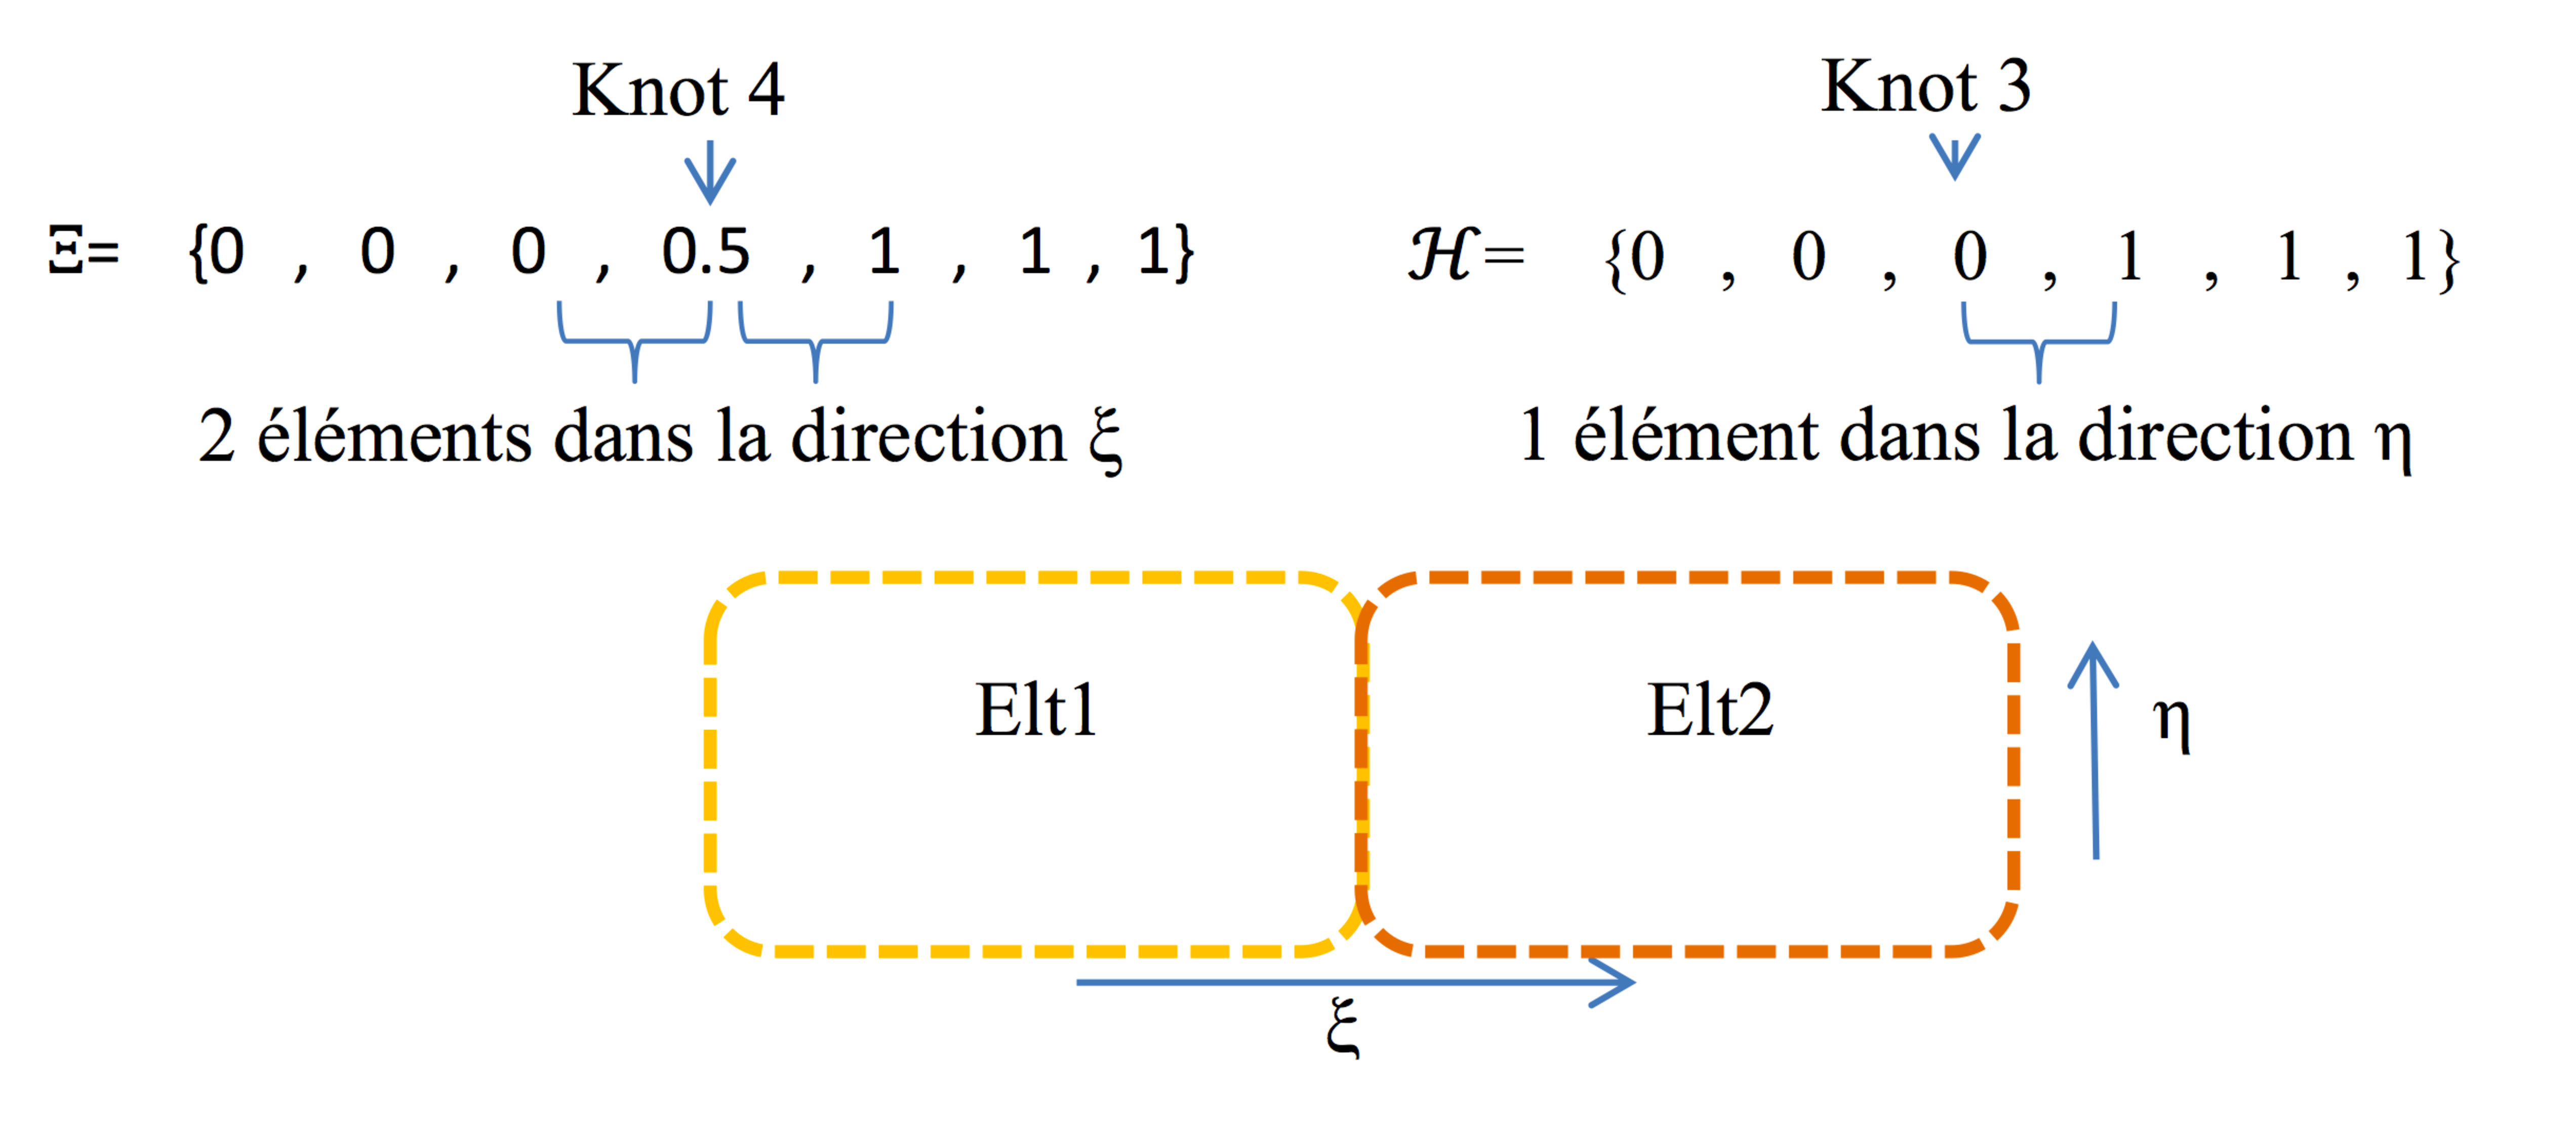
\includegraphics[width=0.5\linewidth]{figures/elem_conn2.pdf}
    \end{center}
  }
\end{frame}

\begin{frame}
  \frametitle{FEA vs IGA}
  \begin{columns}
    \begin{column}{0.4\linewidth}
      \begin{block}{FEA}
        \begin{itemize}
          \item Coordonnées nodales
          \item Type d'élément
          \item Connectivité
          \item Règle d'intégration numérique
        \end{itemize}
      \end{block}
    \end{column}
    \begin{column}{0.55\linewidth}
      \begin{block}{IGA NURBS/B-Splines}
        \begin{itemize}
          \item Coordonnées des points de contrôle
          \item {\bf Poids des points de contrôle (NURBS)}
          \item Degré polynomial
          \item Connectivité
          \item {\bf \emph{knot vectors}}
          \item {\bf \emph{knot spans}}
        \end{itemize}
      \end{block}
    \end{column}
  \end{columns}
\end{frame}

\section{Optimisation}

\begin{frame}
  \frametitle{Optimisation de forme IGA}
  \begin{center}
    \only<1->{\resizebox{0.8\linewidth}{!}{\input{figures/pb_opt_fem}}}
    \only<2>{\resizebox{0.8\linewidth}{!}{%% Creator: Inkscape inkscape 0.48.4, www.inkscape.org
%% PDF/EPS/PS + LaTeX output extension by Johan Engelen, 2010
%% Accompanies image file 'pb_opt_iga.pdf' (pdf, eps, ps)
%%
%% To include the image in your LaTeX document, write
%%   \input{<filename>.pdf_tex}
%%  instead of
%%   \includegraphics{<filename>.pdf}
%% To scale the image, write
%%   \def\svgwidth{<desired width>}
%%   \input{<filename>.pdf_tex}
%%  instead of
%%   \includegraphics[width=<desired width>]{<filename>.pdf}
%%
%% Images with a different path to the parent latex file can
%% be accessed with the `import' package (which may need to be
%% installed) using
%%   \usepackage{import}
%% in the preamble, and then including the image with
%%   \import{<path to file>}{<filename>.pdf_tex}
%% Alternatively, one can specify
%%   \graphicspath{{<path to file>/}}
%%
%% For more information, please see info/svg-inkscape on CTAN:
%%   http://tug.ctan.org/tex-archive/info/svg-inkscape
%%
\begingroup%
  \makeatletter%
  \providecommand\color[2][]{%
    \errmessage{(Inkscape) Color is used for the text in Inkscape, but the package 'color.sty' is not loaded}%
    \renewcommand\color[2][]{}%
  }%
  \providecommand\transparent[1]{%
    \errmessage{(Inkscape) Transparency is used (non-zero) for the text in Inkscape, but the package 'transparent.sty' is not loaded}%
    \renewcommand\transparent[1]{}%
  }%
  \providecommand\rotatebox[2]{#2}%
  \ifx\svgwidth\undefined%
    \setlength{\unitlength}{500bp}%
    \ifx\svgscale\undefined%
      \relax%
    \else%
      \setlength{\unitlength}{\unitlength * \real{\svgscale}}%
    \fi%
  \else%
    \setlength{\unitlength}{\svgwidth}%
  \fi%
  \global\let\svgwidth\undefined%
  \global\let\svgscale\undefined%
  \makeatother%
  \begin{picture}(1,0.24)%
    \put(0,0){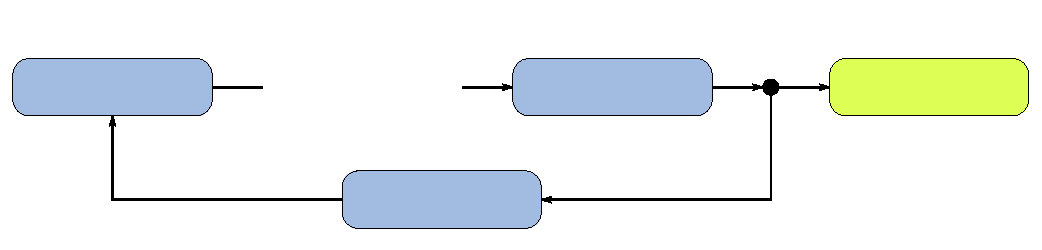
\includegraphics[width=\unitlength]{figures/pb_opt_iga.pdf}}%
    \put(0.34736877,0.15257358){\color[rgb]{0,0,0}\makebox(0,0)[b]{\smash{\large \textbf{\faSmileO~Refinement}}}}%
    \put(0.10835595,0.15959788){\color[rgb]{0,0,0}\makebox(0,0)[b]{\smash{CAD Model}}}%
    \put(0.10768077,0.13785865){\color[rgb]{0,0,0}\makebox(0,0)[b]{\smash{generation}}}%
    \put(0.58820565,0.14911261){\color[rgb]{0,0,0}\makebox(0,0)[b]{\smash{Simulation}}}%
    \put(0.76153551,0.16175593){\color[rgb]{0,0,0}\makebox(0,0)[b]{\smash{\footnotesize Yes}}}%
    \put(0.7226443,0.05406804){\color[rgb]{0,0,0}\makebox(0,0)[b]{\smash{\footnotesize No}}}%
    \put(0.4244494,0.05507856){\color[rgb]{0,0,0}\makebox(0,0)[b]{\smash{Optimization}}}%
    \put(0.42430879,0.0308687){\color[rgb]{0,0,0}\makebox(0,0)[b]{\smash{algorithm}}}%
    \put(0.8915822,0.15097365){\color[rgb]{0,0,0}\makebox(0,0)[b]{\smash{\textit{Optimal Design}}}}%
    %
    \put(0.05,0.225){\color[rgb]{0,0,0}\makebox(0,0)[b]{\Large\smash{\textbf{\texttt{IGA framework:}}}}}%
  \end{picture}%
\endgroup%
}}
  \end{center}
\end{frame}

\begin{frame}
  \frametitle{Optimisation IGA multi-niveau}
  \begin{center}
    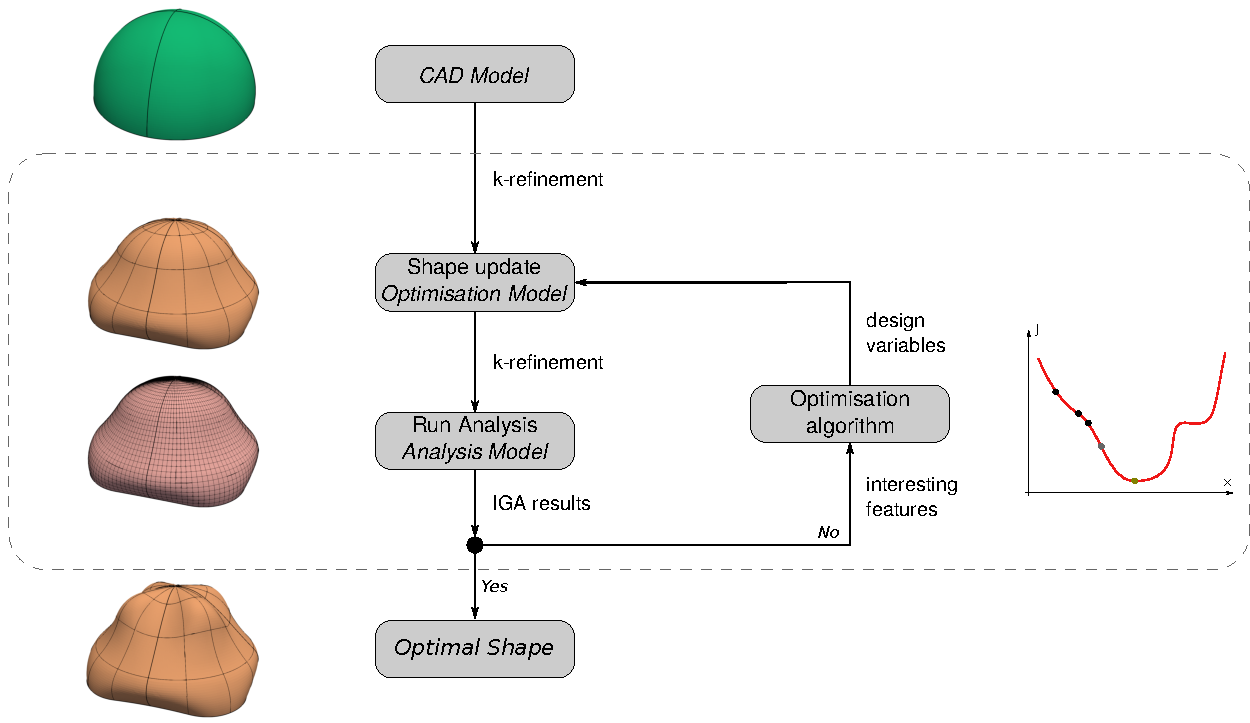
\includegraphics[width=0.8\linewidth]{figures/opt-flowchart.pdf}
  \end{center}
\end{frame}

\begin{frame}
  \frametitle{Variables de design}
  \begin{itemize}
    \item Définir l'espace de design et modifier la forme
  \end{itemize}
  \begin{center}
    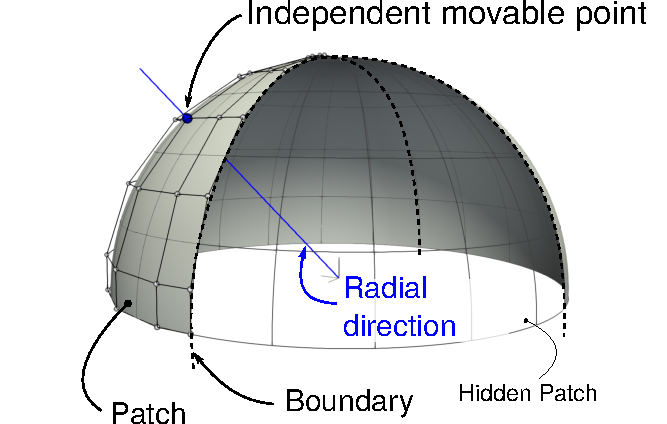
\includegraphics[width=0.4\linewidth]{figures/designvar-shell-free_annotation.pdf}
    \foreach \x in {1,...,5} {
      \only<\x>{\includegraphics[width=0.4\linewidth]{figures/designvar-shell-free-wColor-\x.pdf}}
    }
  \end{center}
\end{frame}

\begin{frame}
  \frametitle{Algorithmes à gradient}
  \begin{itemize}
    \item Problème d'optimisation
    \begin{eqnarray*}
      \textrm{Minimizer} \, f(x) & & \textrm{pour} \,  x \in \mathbb{R}^n \\
      \textrm{Avec les contraintes} \, c_i (x) & = & 0, \forall i \in \mathcal{E} \\
      c_i (x) & \le & 0, \forall i \in \mathcal{F}
    \end{eqnarray*}
    \item Problèmes auto-adjoints : $f, c_i$ \faArrowRight{} compliance, fréquences propres, volume, etc. en élasticité linéaire
    \item $x$ \faArrowRight{} position des points de contrôle
    \item Algorithme d'optimisation à gradients : besoin de calculer $\frac{\textrm{d} f}{\textrm{d} x}$ et $\frac{\textrm{d} c_i}{\textrm{d} x}$ (par défaut en différences finies : {\color{LAMCOSred} nombreuses évaluations de $f$ et $c_i$})
  \end{itemize}
\end{frame}

\begin{frame}
  \frametitle{Sensibilités analytiques}
  \begin{itemize}
    \item Paramétrisation de la forme : $\mathbf{P} := \mathbf{P}(x)$
    \item Passage du modèle de design au modèle d'analyse (raffinement) : $\mathbf{Q} = \mathbf{RP}$
    \item Calcul de structure : $\mathbf{Ku} = \mathbf{F}$
    \item {\color{LAMCOSred} Résolution du problème adjoint : $\mathbf{Ku}^* = \partial f / \partial \mathbf{u}$}
    \item Dérivée du travail adjoint par rapport aux points de contrôle du modèle d'analyse : $\partial W / \partial \mathbf{Q}$
    \item Passage du modèle d'analyse au modèle de design : $\partial W / \partial \mathbf{P} = \mathbf{R}^T \partial W / \partial \mathbf{Q}$
    \item Passage du modèle de design aux variables de design : $\textrm{d} f / \textrm{d} x_i = \partial f / \partial x_i + \partial \mathbf{P} / \partial x_i : \partial W / \partial \mathbf{P}$
  \end{itemize}
  \vspace{5pt}
  Détails : \cite{hirschler_new_2020}
\end{frame}

\section{YETI}

\begin{frame}
  \frametitle{Historique et contributions}
  \begin{itemize}
    \item{2011} abqNURBS : implémentation d'un élément isogéométrique sous Abaqus via subroutine \texttt{UELMAT} (Fortran 77)
    \item{2015} Création d'un code complet autour de l'\texttt{UELMAT} existante (Fortran + Python)
    \item{2019} Coques Kirchhoff-Love + raidisseurs immergés + couplage Mortar + décomposition de domaines FETI \cite{hirschler_dual_2019,hirschler_embedded_2019}
    \item{2022} Solides immergés + couplage Mortar solides 3D + ouverture open-source \cite{guerder_volumetric_2023}
    \item{2024} Analyse sans matrice à quadrature pondérée \cite{cornejo_fuentes_cheap_2023}
    \item{2025+} Couplage de domaines avec recouvrement
  \end{itemize}
\end{frame}

\begin{frame}
  \frametitle{Technologie}
  \begin{itemize}
    \item Bas niveau : routines en Fortran moderne (+ quelques restes en Fortran 77)
    \item Haut niveau : Python
    \item Interfaçage Fortran \faArrowsH{} Python : \texttt{f2py} (package \texttt{numpy})
    \item Construction : \texttt{scikit-build} + \texttt{CMake}
    \item Empaquetage : \texttt{cibuildwheel}
    \item Versionnement \texttt{git} hebergé au LaMCoS (prochainemet \texttt{sourcesup} et/ou \texttt{koda})
    \item Distribution : \texttt{pypi}
    \item Documentation : \texttt{readthedocs.io}
    \item Plateformes supportées : Linux natif ou Linux sous WSL
    \item<2> Windows natif et macOS ? \faArrowRight{} Bienvenue dans l'équipe !
  \end{itemize}
\end{frame}

\begin{frame}
  \frametitle{Travaux pratiques}
  \begin{itemize}
    \item \url{https://lamcosplm.insa-lyon.fr/plugins/git/yeti/tp_csma}
    \item Objectifs
    \begin{itemize}
      \item Comprendre la mise en données d'un problème IGA (knot vectors, spans, degrés, \dots)
      \item Types de raffinements et leur impact sur le système linéaire obtenu
      \item Visualisation des résultats
      \item Mise en données d'un problème d'optimisation de forme basé sur l'IGA
      \item Fonctionnelles dans le cas d'un problème auto-adjoint
      \item Gradients analytiques .vs. différences finies
    \end{itemize}
  \end{itemize}
\end{frame}

\section*{Conclusion}

\begin{frame}
  \frametitle{Bilan}
  \begin{block}{Bilan}
    \begin{itemize}
      \item Lien CAO-calcul impose de retravailler la géométrie (décomposition, reparamétrisation) ou de gérer le trim dans le calcul
      \item Impact important sur un code de calcul existant
      \item Continuité élevée = gains significatifs dans un grand nombre de problèmes : EDP d'ordre supérieur, coques minces, phénomènes haute fréquence, \dots
    \end{itemize}
  \end{block}

  \begin{block}{Intérêts}
    \begin{itemize}
      \item Classes d'applications ciblées
      \item Quantités d'intérêt dérivées (déformations, contraintes, \dots)
      \item Problèmes ou la précision géométrique est essentielle ou la géométrie évolutive
    \end{itemize}
  \end{block}
\end{frame}

\begin{frame}[allowframebreaks]
  \frametitle{Références}
  \printbibliography

\end{frame}

\end{document}
%-------------------------------------------------------------------------------
